\documentclass[11pt]{article}


\usepackage{caption}

\usepackage{kotex}
\usepackage{sectsty}
\usepackage{graphicx}
\usepackage{amsmath}
\usepackage{amssymb}
\usepackage[margin=20mm]{geometry}
\usepackage{listings}
\usepackage{color}
\usepackage{lmodern} % Use a slightly nicer looking font
\usepackage{url} % Proper formatting for URLs
\usepackage{graphicx} % Handle inclusion of non-PDF graphics
\usepackage{subfig} % Allow sub-figures inside a figurexz
\usepackage{enumitem} % Allow lists to pick up numbering where the last list left off
\usepackage[margin=20mm]{geometry}
\usepackage{listings}
\usepackage{color}

\usepackage{setspace}
\usepackage{indentfirst}\setlength\parindent{2em}
\setstretch{1.5} %간격 맞추는 패키지


% Color definitions for source code listings
\definecolor{mygreen}{rgb}{0,0.6,0}
\definecolor{mygray}{rgb}{0.5,0.5,0.5}
\definecolor{mymauve}{rgb}{0.58,0,0.82}

\lstset{ 
  backgroundcolor=\color{white},   % choose the background color; you must add \usepackage{color} or \usepackage{xcolor}
  basicstyle=\footnotesize,        % the size of the fonts that are used for the code
  breakatwhitespace=false,         % sets if automatic breaks should only happen at whitespace
  breaklines=true,                 % sets automatic line breaking
  captionpos=b,                    % sets the caption-position to bottom
  commentstyle=\color{mygreen},    % comment style
  deletekeywords={...},            % if you want to delete keywords from the given language
  escapeinside={\%*}{*)},          % if you want to add LaTeX within your code
  extendedchars=true,              % lets you use non-ASCII characters; for 8-bits encodings only, does not work with UTF-8
  frame=single,	                   % adds a frame around the code
  keepspaces=true,                 % keeps spaces in text, useful for keeping indentation of code (possibly needs columns=flexible)
  keywordstyle=\color{blue},       % keyword style
  otherkeywords={*,...},           % if you want to add more keywords to the set
  numbers=left,                    % where to put the line-numbers; possible values are (none, left, right)
  numbersep=5pt,                   % how far the line-numbers are from the code
  numberstyle=\tiny\color{mygray}, % the style that is used for the line-numbers
  rulecolor=\color{black},         % if not set, the frame-color may be changed on line-breaks within not-black text (e.g. comments (green here))
  showspaces=false,                % show spaces everywhere adding particular underscores; it overrides 'showstringspaces'
  showstringspaces=false,          % underline spaces within strings only
  showtabs=false,                  % show tabs within strings adding particular underscores
  stepnumber=2,                    % the step between two line-numbers. If it's 1, each line will be numbered
  stringstyle=\color{mymauve},     % string literal style
  tabsize=2,	                   % sets default tabsize to 2 spaces
  title=\lstname                   % show the filename of files included with \lstinputlisting; also try caption instead of title
}


% Margins
\topmargin=-0.45in
\evensidemargin=0in
\oddsidemargin=0in
\textwidth=6.5in
\textheight=9.0in
\headsep=0.25in


\title{Fourier Transform Homework 5}
\author{MinWook Kang}
\date{\today}

\begin{document}
\maketitle
\pagebreak

% Optional TOC
% \tableofcontents
% \pagebreak


%--Paper--



\section{Differentiation of Functions} 
\subsection{Problem Recognition} 
$x \in [0, 2\pi)$내의 25개의 포인트를 정하여, FFT를 통해 함수를 미분하는 문제이다. 함수는 다음과 같다.

\begin{enumerate}
    \item \begin{equation} u(x) = \max\left\{0, 1 - \frac{|x - \pi|}{2}\right\}
\end{equation}

       \item  \begin{equation}
e^{\sin x}
\end{equation}
\end{enumerate}


이때, 우리가 FFT를 이용하여 구한 미분값과 exact solution을 비교하고 정확성을 확인하는 문제이다. 
\subsection{Development of a solution} 
우선 FFT의 Spectral Differentiation을 이용하려면, 우리가 구할려고 하는 함수가 해당 범위에서 주기성을 이루는지를 확인해야 한다. 각각의 함수에 대해 범위를 지정해주고 그것에 대한 그래프를 먼저 그려보고, 그 그래프가 주기성을 가지면, 아래의 절차를 통해 함수의 미분값을 구할 수 있다.

우선, 주기 함수 $u(x)$에 대해, $u_j$는 N번 샘플링 된 이산화 격자 점, $x_j =.0, 1, ... , N - 1$의 함수값이고, 역 이산화 푸리에 변환에 따르면, 
\begin{equation}
u_j = \frac{\Delta k}{2\pi} \sum_{l = 0}^{N - 1} \hat u_l e^{i x_j k_l}
\end{equation}
그리고 $v_j$를 $u'(x_j)$로 두면, 위의 식으로부터 우리는 아래를 얻는다.
\begin{equation}
v_j = \frac{\Delta k}{2\pi} \sum_{l = 0}^{N - 1}
\underbrace{i k_l \hat u_l}_{\hat v_l}
e^{i x_j k_l}
= \frac{\Delta k}{2\pi} \sum_{l = 0}^{N - 1} \hat v_l e^{i x_j k_l}
\end{equation}
따라서 1차 미분 값은 $\hat v_l = ik_l\hat u_l$이고 이는 푸리에 계수  의 역 DFT이다. 마찬가지 방식으로 2차 미분 값을 구하게 되면,
\begin{equation}
w_j = \frac{\Delta k}{2\pi} \sum_{l = 0}^{N - 1}
\underbrace{-k_l^2 \hat u_l}_{\hat w_l}
e^{i x_j k_l}
= \frac{\Delta k}{2\pi} \sum_{l = 0}^{N - 1} \hat w_l e^{i x_j k_l}
\end{equation}
이고, 2차 미분 값 $w_j = u''(x_j)$ 그리고 이는 $\hat w_l = -k_l^2 \hat u_l$로,  푸리에 계수의 역 DFT이다. 우리는 $v_j$와  $w_j$를 푸리에 계수의 역 DFT로 구했고, 이것을 통해 함수의 1차, 2차 미분값을 찾을 것이다. 여기서 홀수 N에 대해서 $k_l$은 $l = 0, 1, ... M, M + 1, ..., N - 2, N - 1$ 일때 $k = 0, \Delta k, ... ,M\Delta k, -M\Delta k, ... , -2\Delta k, -\Delta k$로 추정한다. 여기서 M은 우리가 구현할 파이썬에서 int(N/2)에 해당한다.

N = 25로 두고 주어진 범위, $x \in [0, 2\pi)$에서 L과 xj를 정의 한다. 그리고 첫번째 함수는 max 함수에 따라 $1 - \frac{|x - \pi|}{2}$가 0 보다 커지기 전까지 0을 나타내는 함수이다. 1번 함수를 그대로 $u_j$에 정의하여, 1차와 2차 미분 방정식을 풀어주면 다음과 같다.

\begin{lstlisting}[language=Python]
N = 25
xlim = [0, 2 * np.pi]
L  = xlim[1] - xlim[0]
xj = np.linspace(*xlim, N + 1)[:-1]

#definition of function 1
uj = [max(0, 1 - (abs(x - np.pi)/ 2)) for x in xj]
Uj = fft.fft(uj)
kj = np.hstack([
    np.arange(0,   N/2),     # k > 0 domain
    np.arange(-int(N/2), 0), # k < 0 domain
]) * 2*np.pi/L

# 1st-order derivatives
Vj = 1j * kj * Uj
vj = fft.ifft(Vj)

# 2nd-order derivatives
Wj = -1 * kj**2 * Uj
wj = fft.ifft(Wj)

# exact solution and vj.real solution plot
plt.figure(figsize=[11, 4])

plt.subplot(1, 2, 1)
plt.plot(xj, vj.real, "--r")
plt.legend(["$u'(x_j)$", "$v_j$"])
plt.xlabel("$x$")
plt.title("$u'(x)$")
plt.grid()

plt.subplot(1, 2, 2)
plt.plot(xj, wj.real, "--r")
plt.legend(["$u''(x_j)$", "$w_j$"])
plt.xlabel("$x$")
plt.title("$u''(x)$")
plt.grid()

plt.tight_layout()
plt.savefig("Differntiation_1.pdf")
\end{lstlisting}

\begin{figure}[!ht]
  \centering
  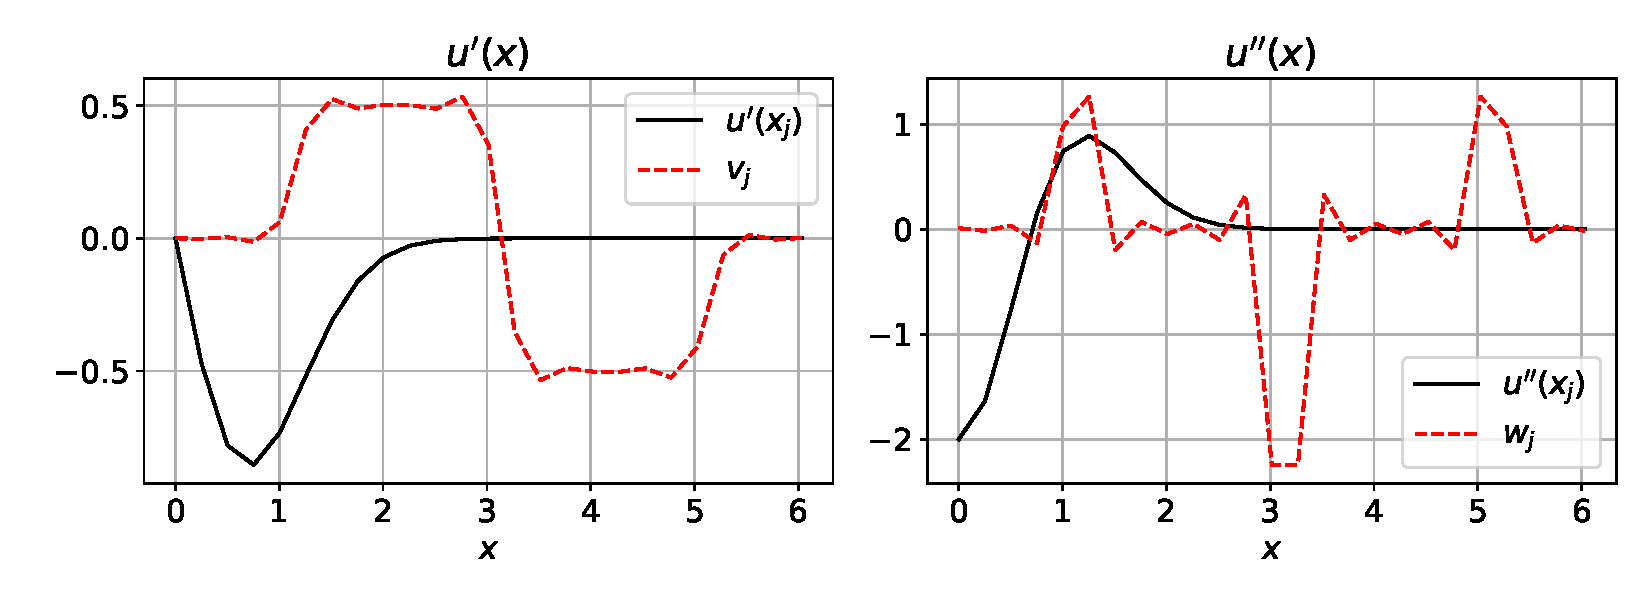
\includegraphics[width=1\textwidth]{Differntiation_1.pdf}
  \caption{Derivatives of $ \max\left\{0, 1 - \frac{|x - \pi|}{2}\right\}$}
\end{figure}

이때 1번 함수의 실제 미분값을 확인하려면 본래 함수를 그려준뒤, 직접 확인할 수 있다. 
\begin{lstlisting}[language=Python]
plt.figure(figsize = (10, 5))
x = np.linspace(0, 2 * np.pi, 100)
plt. plot(x, [max(0, 1 - (abs(x - np.pi)/ 2)) for x in x], '-r')
plt.savefig("Max_graph.pdf")

c = [x for x in x if max(0, 1 - (abs(x - np.pi)/ 2)) != 0]
#u'(x)
uprime = (max(0, 1 - (abs(np.pi - np.pi)/ 2) - max(0, 1 - (abs(c[0] - np.pi)/ 2))) / (np.pi - c[0]))
print(f"uprime: {uprime}")
print(f"uprime = {uprime}, x min = {c[0]}")
print(f"uprime = {uprime}, x middle = {(c[0] + c[-1]) / 2}")
print(f"uprime = {-1 * uprime}, x max = {c[-1]}")


#Output:
uprime: 0.5
uprime = 0.5, x min = 1.1423973285781066
uprime = 0.5, x middle = 3.1415926535897936
uprime = -0.5, x max = 5.14078797860148

\end{lstlisting}

\begin{figure}[!ht]
  \centering
  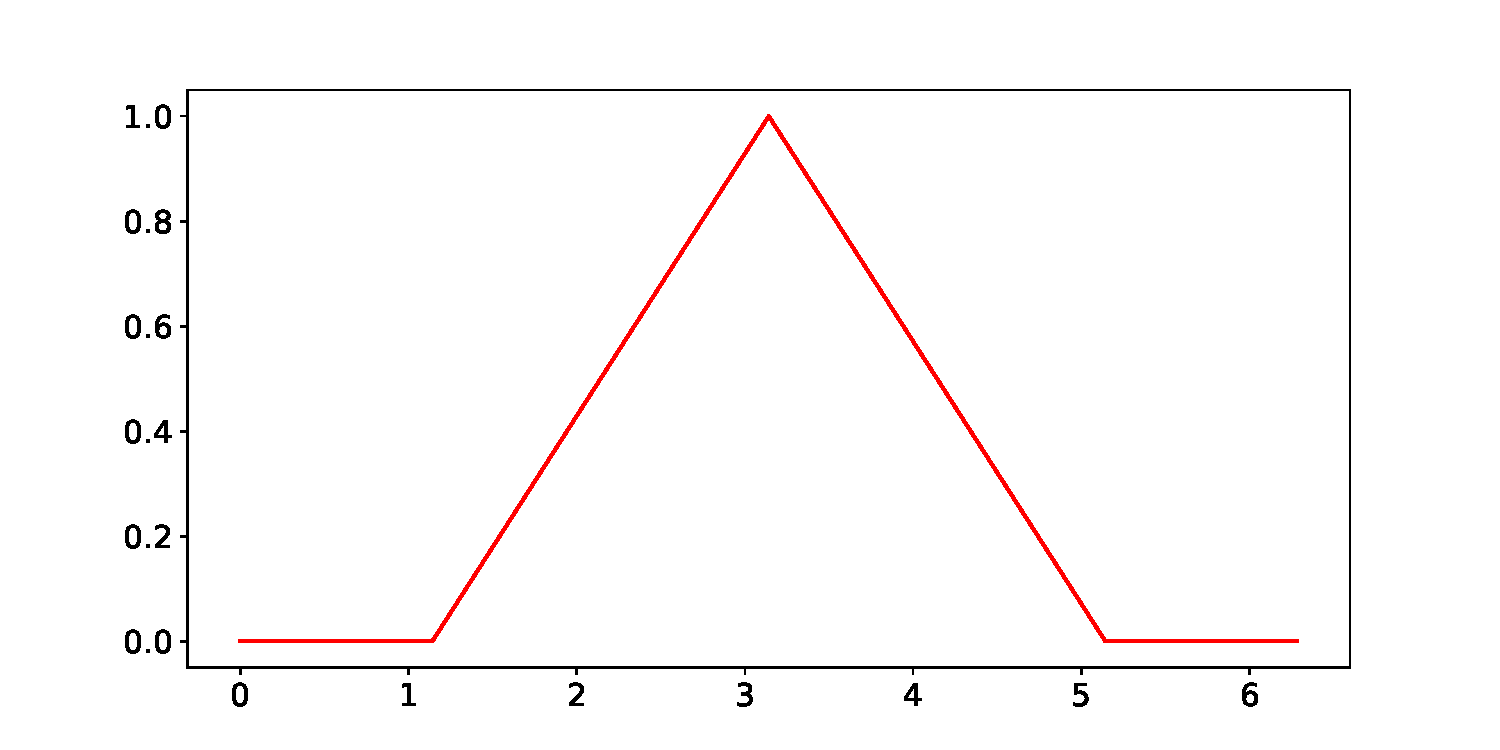
\includegraphics[width=1\textwidth]{Max_graph.pdf}
  \caption{1st $u(x)$}
\end{figure}
이 그래프의 1차 미분 그래프는 $1.1423973285781066 \le x  < 3.1415926535897936$ 까지는 0.5이며 $1.1423973285781066 <  x  \le 3.1415926535897936$ 는 -0.5이고 나머지는 0 인 함수이다. 이를 그래프로 나타내면,

\begin{lstlisting}[language=Python]
def f(x):
    if 1.1417689472092518 <= x and x < 3.141592653589793:
        return 0.5
    elif  x >= 3.141592653589793 and x < 5.141416359970335:
        return -0.5
    else:
        return 0
plt.figure(figsize = (10, 5))
x = np.linspace(0, 2 * np.pi, 10000)
plt.plot(x, [f(x) for x in x], '-r')
plt.savefig("Max_graph_uprime.pdf")
\end{lstlisting}

\begin{figure}[!ht]
  \centering
  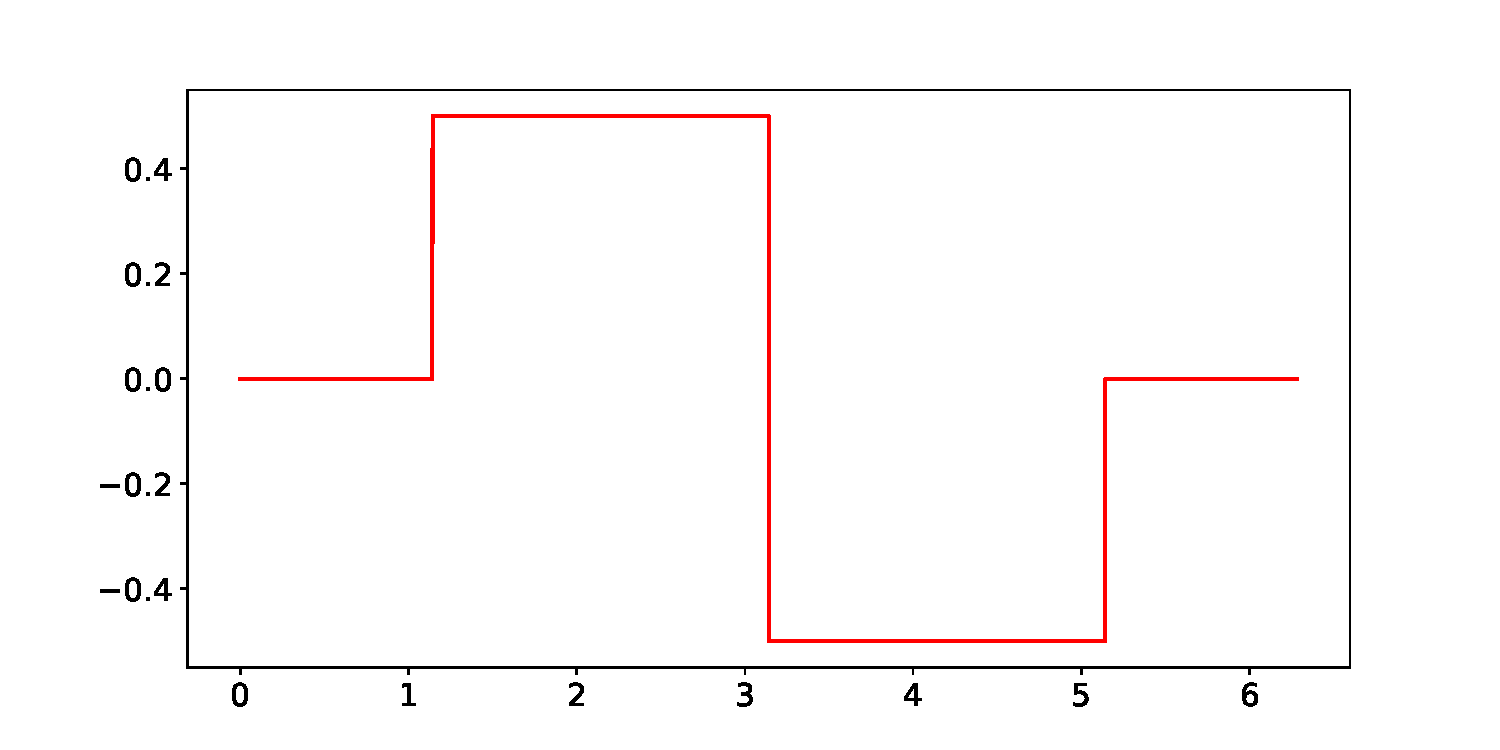
\includegraphics[width=1\textwidth]{Max_graph_uprime.pdf}
  \caption{1st function, u'(x)}
\end{figure}

u의 이차 미분값은 x = 1.1417689472092518, 3.141592653589793, 5.141416359970335 일때 무한한 값을 가지므로 이를 그래프로 그리면 다음과 같다.

\begin{lstlisting}[language=Python]
import sys
def g(x):
    if x == 1.1417689472092518:
        return sys.maxsize
    if x == 3.141592653589793:
        return -1 * sys.maxsize
    if x == 5.141416359970335:
        return sys.maxsize
    else: 
        return 0
plt.figure(figsize = (10, 5))
x = np.linspace(0, 2 * np.pi, 1000)
print()
x = np.append(x, np.array([1.1417689472092518, 3.141592653589793,5.141416359970335]))
plt. plot(x, [g(x) for x in x], '.r')
#print(1.1417689472092518 in x)
plt.savefig("Max_graph_u_two_prime.pdf")
\end{lstlisting}
    
\begin{figure}[!ht]
  \centering
  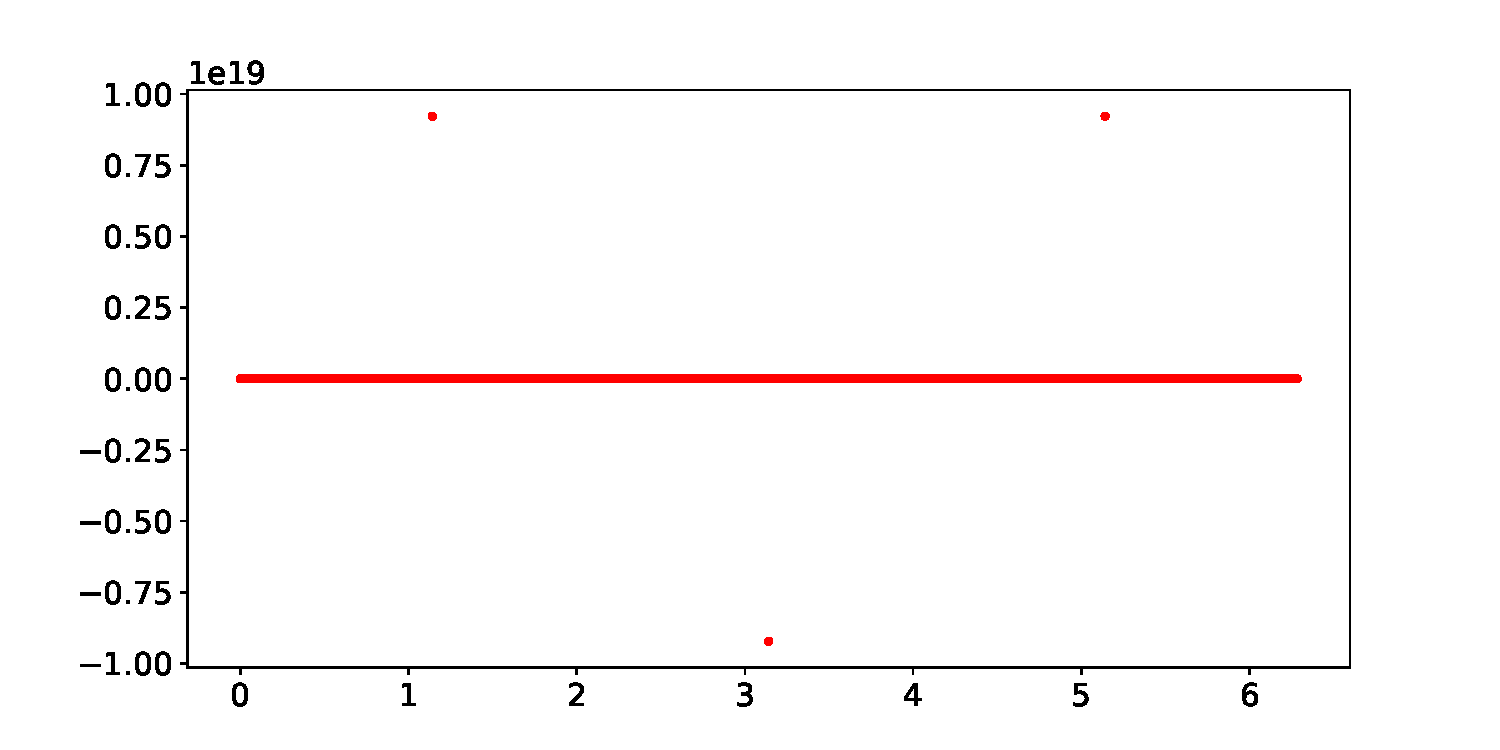
\includegraphics[width=1\textwidth]{Max_graph_u_two_prime.pdf}
  \caption{1st function, u"(x)}
\end{figure}

따라서 오차 값을 계산하면 다음과 같다.

\begin{lstlisting}[language=Python]
# Compare the exact solutions and vj, uj
print("-"*70)
print("1st-order derivatives accuracy")
print("-"*70)
error1 = [f(x) for x in xj] - vj.real
for i, err in enumerate(error1):
    print(f"if x = {xj[i]:.8f}, u - vj: {err}")
print("-"*70)
print("2st-order derivatives accuracy")
print("-"*70)
error2 = [g(x) for x in xj] - wj.real
for i, err in enumerate(error2):
    print(f"if x = {xj[i]:.8f}, u - wj: {err}")
    
#Output:
----------------------------------------------------------------------
1st-order derivatives accuracy
----------------------------------------------------------------------
if x = 0.00000000, u - vj: 8.066242429609187e-17
if x = 0.25132741, u - vj: 0.0014631148894537738
if x = 0.50265482, u - vj: -0.004311303416735122
if x = 0.75398224, u - vj: 0.013115501880781685
if x = 1.00530965, u - vj: -0.06158369933473708
if x = 1.25663706, u - vj: 0.09049064073186014
if x = 1.50796447, u - vj: -0.024866724181648037
if x = 1.75929189, u - vj: 0.01017010280031344
if x = 2.01061930, u - vj: -0.003413769806141609
if x = 2.26194671, u - vj: -0.0023533647118346712
if x = 2.51327412, u - vj: 0.0113066175021313
if x = 2.76460154, u - vj: -0.03450964062384332
if x = 3.01592895, u - vj: 0.14848380535260197
if x = 3.26725636, u - vj: -0.14848380535259997
if x = 3.51858377, u - vj: 0.03450964062384321
if x = 3.76991118, u - vj: -0.011306617502133132
if x = 4.02123860, u - vj: 0.0023533647118360035
if x = 4.27256601, u - vj: 0.003413769806141498
if x = 4.52389342, u - vj: -0.010170102800313607
if x = 4.77522083, u - vj: 0.024866724181647926
if x = 5.02654825, u - vj: -0.0904906407318613
if x = 5.27787566, u - vj: 0.06158369933473793
if x = 5.52920307, u - vj: -0.013115501880782787
if x = 5.78053048, u - vj: 0.004311303416735512
if x = 6.03185789, u - vj: -0.0014631148894539336
----------------------------------------------------------------------
2st-order derivatives accuracy
----------------------------------------------------------------------
if x = 0.00000000, u - wj: -0.010268797450089408
if x = 0.25132741, u - wj: 0.01458431707515821
if x = 0.50265482, u - wj: -0.03535583584850755
if x = 0.75398224, u - wj: 0.13026928537371504
if x = 1.00530965, u - wj: -0.9810809508067928
if x = 1.25663706, u - wj: -1.2637731565649577
if x = 1.50796447, u - wj: 0.19731141844112352
if x = 1.75929189, u - wj: -0.0700932483636727
if x = 2.01061930, u - wj: 0.04470475641843592
if x = 2.26194671, u - wj: -0.05181049056075088
if x = 2.51327412, u - wj: 0.10201809229407806
if x = 2.76460154, u - wj: -0.3260604370764809
if x = 3.01592895, u - wj: 2.2444206483437013
if x = 3.26725636, u - wj: 2.244420648343697
if x = 3.51858377, u - wj: -0.3260604370764926
if x = 3.76991118, u - wj: 0.10201809229408236
if x = 4.02123860, u - wj: -0.0518104905607413
if x = 4.27256601, u - wj: 0.04470475641842299
if x = 4.52389342, u - wj: -0.07009324836366318
if x = 4.77522083, u - wj: 0.19731141844111236
if x = 5.02654825, u - wj: -1.2637731565649473
if x = 5.27787566, u - wj: -0.9810809508067968
if x = 5.52920307, u - wj: 0.13026928537371404
if x = 5.78053048, u - wj: -0.03535583584850443
if x = 6.03185789, u - wj: 0.014584317075156346
    \end{lstlisting}
    
    

\pagebreak 
그리고 2번 함수같은 경우는, $sin(x)$가 지수함수 안에 들어간 형태로 마찬가지로 $u_j$에 대입하게 되면,
\begin{lstlisting}[language=Python]
N = 25
xlim = [0, 2 * np.pi]
L  = xlim[1] - xlim[0]
xj = np.linspace(*xlim, N + 1)[:-1]

#definition of function 2
uj = [np.exp(np.sin(x)) for x in xj]
Uj = fft.fft(uj)
kj = np.hstack([
    np.arange(0,   N/2),     # k > 0 domain
    np.arange(-int(N/2), 0), # k < 0 domain
]) * 2*np.pi/L

# 1st-order derivatives
Vj = 1j * kj * Uj
vj = fft.ifft(Vj)

# 2nd-order derivatives
Wj = -1 * kj**2 * Uj
wj = fft.ifft(Wj)

# exact solution and vj.real solution plot
plt.figure(figsize=[11, 4])

plt.subplot(1, 2, 1)
plt.plot(xj, np.cos(xj) * np.exp(np.sin(xj)), "-k",
         xj, vj.real, "--r")

plt.legend(["$u'(x_j)$", "$v_j$"])
plt.xlabel("$x$")
plt.title("$u'(x)$")
plt.grid()

plt.subplot(1, 2, 2)
plt.plot(xj, ((np.cos(xj))**2 - np.sin(xj)) * np.exp(np.sin(xj)), "-k",
         xj, wj.real, "--r")
plt.legend(["$u''(x_j)$", "$w_j$"])
plt.xlabel("$x$")
plt.title("$u''(x)$")
plt.grid()
plt.tight_layout()
plt.savefig("Differntiation_2.pdf")


# Compare the exact solutions and vj, uj
print("-"*70)
print("1st-order derivatives accuracy")
print("-"*70)
error1 = np.cos(xj) * np.exp(np.sin(xj)) - vj.real 
for i, err in enumerate(error1):
    print(f"if x = {xj[i]:.8f}, u - wj: {err}")
print("-"*70)
print("2st-order derivatives accuracy")
print("-"*70)
error2 = ((np.cos(xj))**2 - np.sin(xj)) * np.exp(np.sin(xj)) - wj.real 
for i, err in enumerate(error2):
    print(f"if x = {xj[i]:.8f}, u - wj: {err}")
    
#Output
----------------------------------------------------------------------
1st-order derivatives accuracy
----------------------------------------------------------------------
if x = 0.00000000, u - wj: 9.999778782798785e-13
if x = 0.25132741, u - wj: -1.0031975250512914e-12
if x = 0.50265482, u - wj: 9.9298347322474e-13
if x = 0.75398224, u - wj: -9.636735853746359e-13
if x = 1.00530965, u - wj: 9.128253708468037e-13
if x = 1.25663706, u - wj: -8.423262087831063e-13
if x = 1.50796447, u - wj: 7.576994587310537e-13
if x = 1.75929189, u - wj: -6.540323838066797e-13
if x = 2.01061930, u - wj: 5.362377208939506e-13
if x = 2.26194671, u - wj: -4.1611158962950867e-13
if x = 2.51327412, u - wj: 2.877698079828406e-13
if x = 2.76460154, u - wj: -1.5476508963274682e-13
if x = 3.01592895, u - wj: 2.731148640577885e-14
if x = 3.26725636, u - wj: 9.725553695716371e-14
if x = 3.51858377, u - wj: -2.1471713296250527e-13
if x = 3.76991118, u - wj: 3.26183524634871e-13
if x = 4.02123860, u - wj: -4.330424907550423e-13
if x = 4.27256601, u - wj: 5.312417172831374e-13
if x = 4.52389342, u - wj: -6.192407697724889e-13
if x = 4.77522083, u - wj: 7.001239865633835e-13
if x = 5.02654825, u - wj: -7.737976925881185e-13
if x = 5.27787566, u - wj: 8.387457395286901e-13
if x = 5.52920307, u - wj: -8.93729534823251e-13
if x = 5.78053048, u - wj: 9.401368572525826e-13
if x = 6.03185789, u - wj: -9.777734177873754e-13
----------------------------------------------------------------------
2st-order derivatives accuracy
----------------------------------------------------------------------
if x = 0.00000000, u - wj: 9.059419880941277e-14
if x = 0.25132741, u - wj: 3.11972669919669e-14
if x = 0.50265482, u - wj: -1.7502665983215593e-13
if x = 0.75398224, u - wj: 3.106404022901188e-13
if x = 1.00530965, u - wj: -4.531930386519889e-13
if x = 1.25663706, u - wj: 6.09734485124136e-13
if x = 1.50796447, u - wj: -7.407408020299044e-13
if x = 1.75929189, u - wj: 8.477663016037695e-13
if x = 2.01061930, u - wj: -9.51017042893909e-13
if x = 2.26194671, u - wj: 1.0146328222049306e-12
if x = 2.51327412, u - wj: -1.0266093530830744e-12
if x = 2.76460154, u - wj: 1.0239586956117819e-12
if x = 3.01592895, u - wj: -1.0091927293842673e-12
if x = 3.26725636, u - wj: 9.742207041085749e-13
if x = 3.51858377, u - wj: -9.218181773462675e-13
if x = 3.76991118, u - wj: 8.505418591653324e-13
if x = 4.02123860, u - wj: -7.844835892001356e-13
if x = 4.27256601, u - wj: 7.344680419407723e-13
if x = 4.52389342, u - wj: -6.808442698513772e-13
if x = 4.77522083, u - wj: 6.167288901792745e-13
if x = 5.02654825, u - wj: -5.47950573803746e-13
if x = 5.27787566, u - wj: 4.745648318760232e-13
if x = 5.52920307, u - wj: -3.872457909892546e-13
if x = 5.78053048, u - wj: 2.836619827917275e-13
if x = 6.03185789, u - wj: -1.829647544582258e-13
\end{lstlisting}

\begin{figure}[!ht]
  \centering
  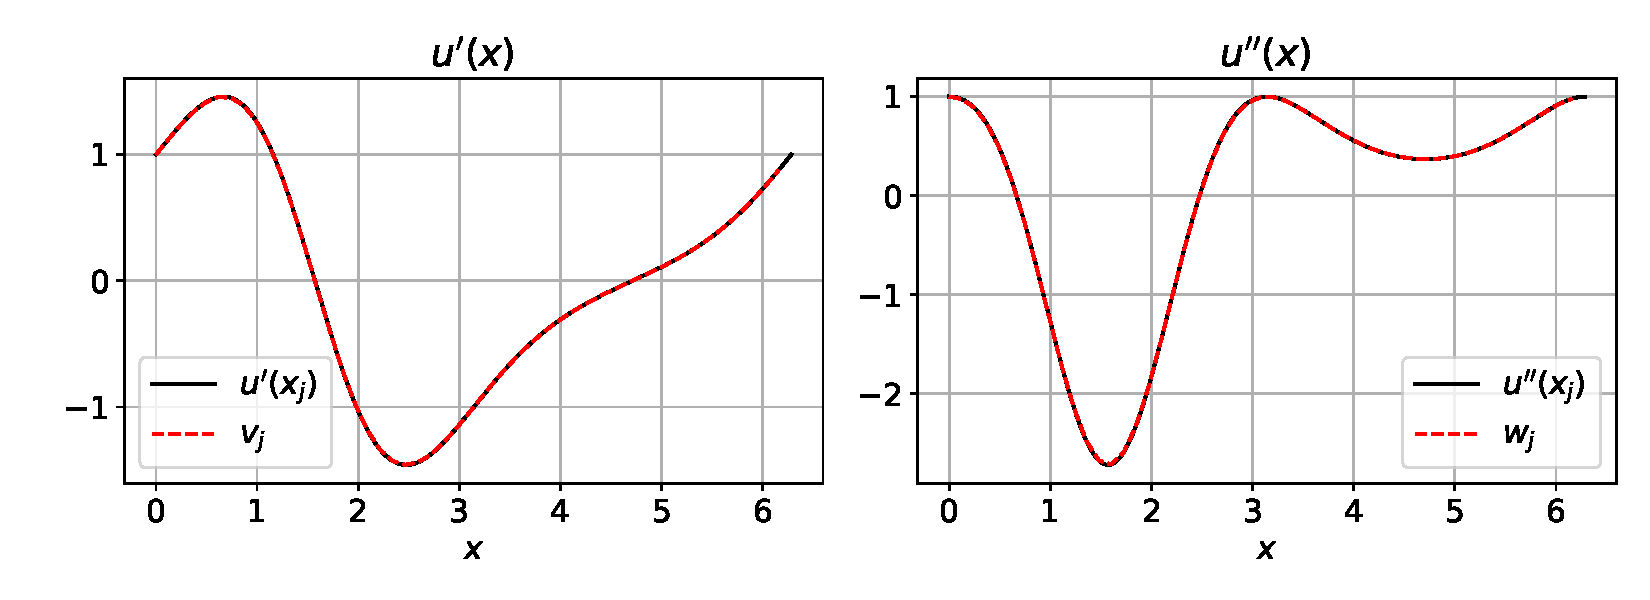
\includegraphics[width=1\textwidth]{Differntiation_2.pdf}
  \caption{Derivatives of $e^{sin(x)}$}
\end{figure}

\subsection{Execution and Assessment}
실제로 미분한 Exact Solution과 FFT를 이용하여 구한 미분 값의 오차가 매우 작은 것을 볼 수 있다. 이것으로 우리는, 미분이 쉽게 불가능한 함수도, FFT와 Spectrum Differentiaion을 통해 미분값을 찾을 수 있다는 것을 보았다.

\pagebreak












\section{1D Wave Solution}
\subsection{Problem Recognition} 
\begin{enumerate}
    \item 1D wave program에서 초기 가우스 펄스가 오른쪽으로 전파하도록 수정한다.
\begin{equation}
u(0, x) = -\exp(-200 x^2)
\end{equation}
    \item 처음에 다음과 같이 하나의 펄스가 주어지도록 프로그램을 수정한다.
    \begin{equation}
u_1(0, x) = -\exp(-200 (x + 0.5)^2)
\end{equation}
이는 오른쪽으로 전파되고 다른 하나는 다음과 같이 주어지도록 수정하면
    \begin{equation}
u_2(0, x) = \exp(-200 (x - 0.5)^2),
\end{equation}
왼쪽으로 전파된다. 두 펄스가 서로 교차할 때 어떤 일이 일어나는지 확인한다.
\end{enumerate}

\subsection{Development of a solution} 
이 문제의 경우 주어진 코드에서 $u$에 대해 우리가 원하는 값만큼 수정하면 된다. 따라서 미리 알려진 코드에서,

\begin{lstlisting}[language=Python]
N = 121 # number of grid points in x
xlim = [-1, 1] # bound of x
L  = xlim[1] - xlim[0]
xj = np.linspace(*xlim, N + 1)[:-1]
kj = np.hstack([
    np.arange(0,   N/2),     # k > 0 domain
    np.arange(-int(N/2), 0), # k < 0 domain
]) * 2*np.pi/L

dt = 4 / N**2 # stability criterion is a whole different subject...
tmax = 4      # the maximum time to integrate
datadump_freq = int(0.01 / dt) # intermediate data dump frequency
outer_loop_count = int(tmax/dt / datadump_freq)

uj = np.exp(-200 * xj**2)            # u(  0, x)
uj_old = np.exp(-200 * (xj - dt)**2) # u(-Dt, x)

# time and u data containers
t_data = [dt] * (1 + outer_loop_count)
u_data = [uj] * (1 + outer_loop_count)

for i in range(outer_loop_count):
    t_data[i] *= i * datadump_freq
    u_data[i]  = uj

    for _ in range(datadump_freq):
        Uj = fft.fft(uj)
        Wj = -kj**2 * Uj       # approximation for u_xx
        wj = fft.ifft(Wj).real # remove the imaginary part, which should all be zeros
        uj_old, uj = uj, 2*uj - uj_old + dt**2*wj

t_data[-1] *= i * datadump_freq
u_data[-1]  = uj

#plot
fig, ax = plt.subplots(figsize=(7, 7), ncols=1)

pos = ax.imshow(u_data, interpolation='none', origin='lower', cmap='viridis',
           extent=np.hstack(([xj[0], xj[-1]], [t_data[0], t_data[-1]])),
           aspect='auto')
fig.colorbar(pos, ax=ax, location='right', anchor=(0, 0.3), shrink=0.7,
             label="$u(t, x)$")
ax.set_xlabel("$x$")
ax.set_ylabel("$t$")

plt.savefig("1d_Wave_Solution.pdf")
\end{lstlisting}
에서 공간 영역이 $-1 \le x < 1$일때, 정수 n에 대해 주기적인 $u(t, x) = u(t, x + 2n)$의 초기조건은 다음과 같이 가정하였다.
\begin{equation}
u(0, x) = \exp(-200 x^2)
\end{equation}
이는 곧 위 코드의 
\begin{lstlisting}[language=Python]
uj = np.exp(-200 * xj**2)            # u(  0, x)
uj_old = np.exp(-200 * (xj - dt)**2) # u(-Dt, x)
\end{lstlisting}
이 두 줄을 초기값에 맞게 수정하면 된다. 따라서 우리가 만들 1번의 조건에서의 함수는, 5번식이기 때문에, 다음과 같이 수정될 수 있다.
\begin{lstlisting}[language=Python]
uj = -1 * np.exp(-200 * xj**2)            # - u(  0, x)
uj_old = -1 * np.exp(-200 * (xj - dt)**2) # - u(-Dt, x)
\end{lstlisting}
이 부분만 수정하여 위에 있는 예제 코드에 적용해 그래프를 그리게 되면,


\begin{figure}[!ht]
  \centering
  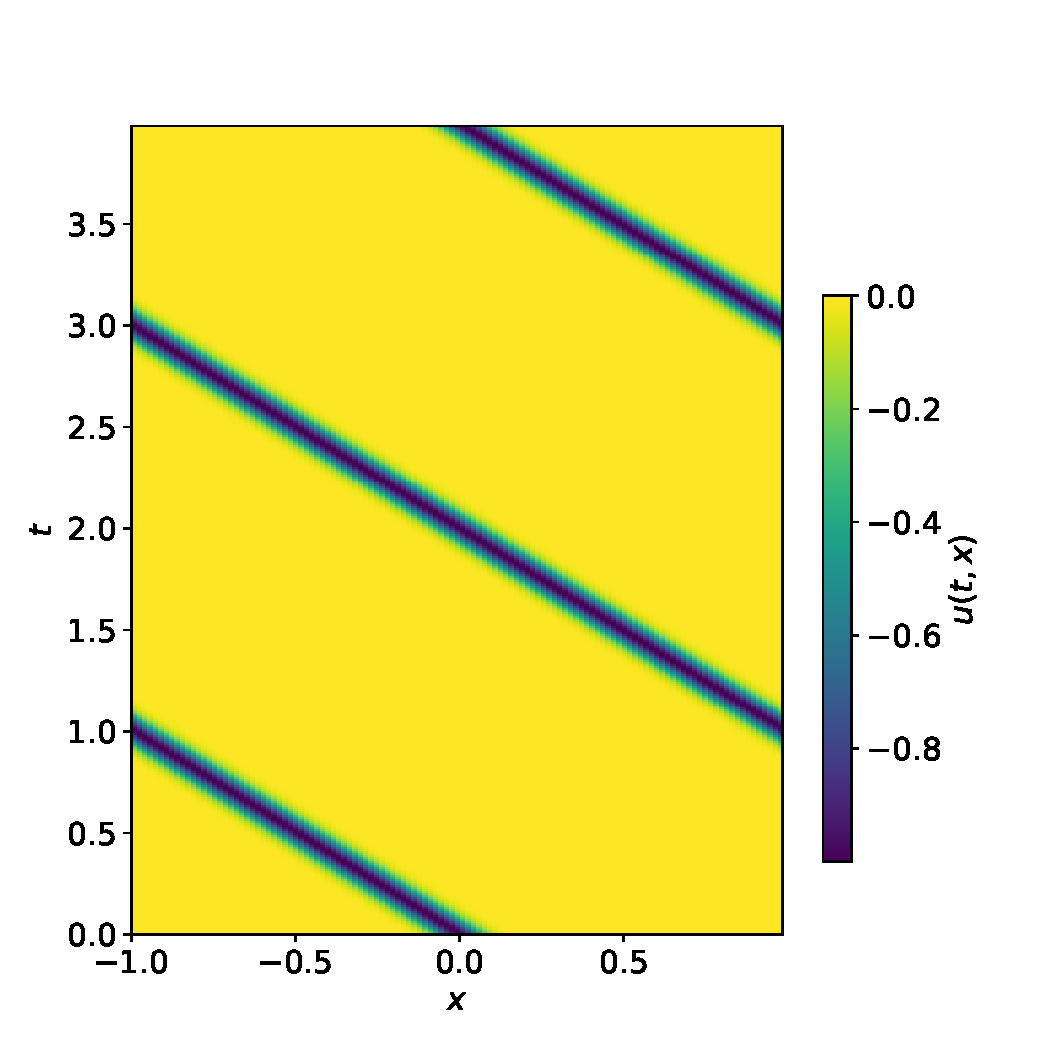
\includegraphics[width=0.8\textwidth]{1d_Wave_Solution.pdf}
  \caption{initial 1 Gaussian Pulse}
\end{figure}

마찬가지로, 2번 문제의 $u_1$의 코드는 다음과 같이 수정된다.
\begin{lstlisting}[language=Python]
uj = -1 * np.exp(-200 * (xj + 0.5)**2)            # - u(  0, x)
uj_old = -1 * np.exp(-200 * ((xj + 0.5) - dt)**2) # - u(-Dt, x)
\end{lstlisting}
그래프를 그리게 되면,

\begin{figure}[!ht]
  \centering
  \includegraphics[width=0.8\textwidth]{1d_Wave_Solution2_u1.pdf}
  \caption{initial 2 Gaussian Pulse $u_1$}
\end{figure}
그리고 2번 문제의 $u_2$ 또한 동일하게 진행하면,
\begin{lstlisting}[language=Python]
uj = np.exp(-200 * (xj - 0.5)**2)            # - u(  0, x)
uj_old = np.exp(-200 * ((xj - 0.5) - dt)**2) # - u(-Dt, x)
\end{lstlisting}

\begin{figure}[!ht]
  \centering
  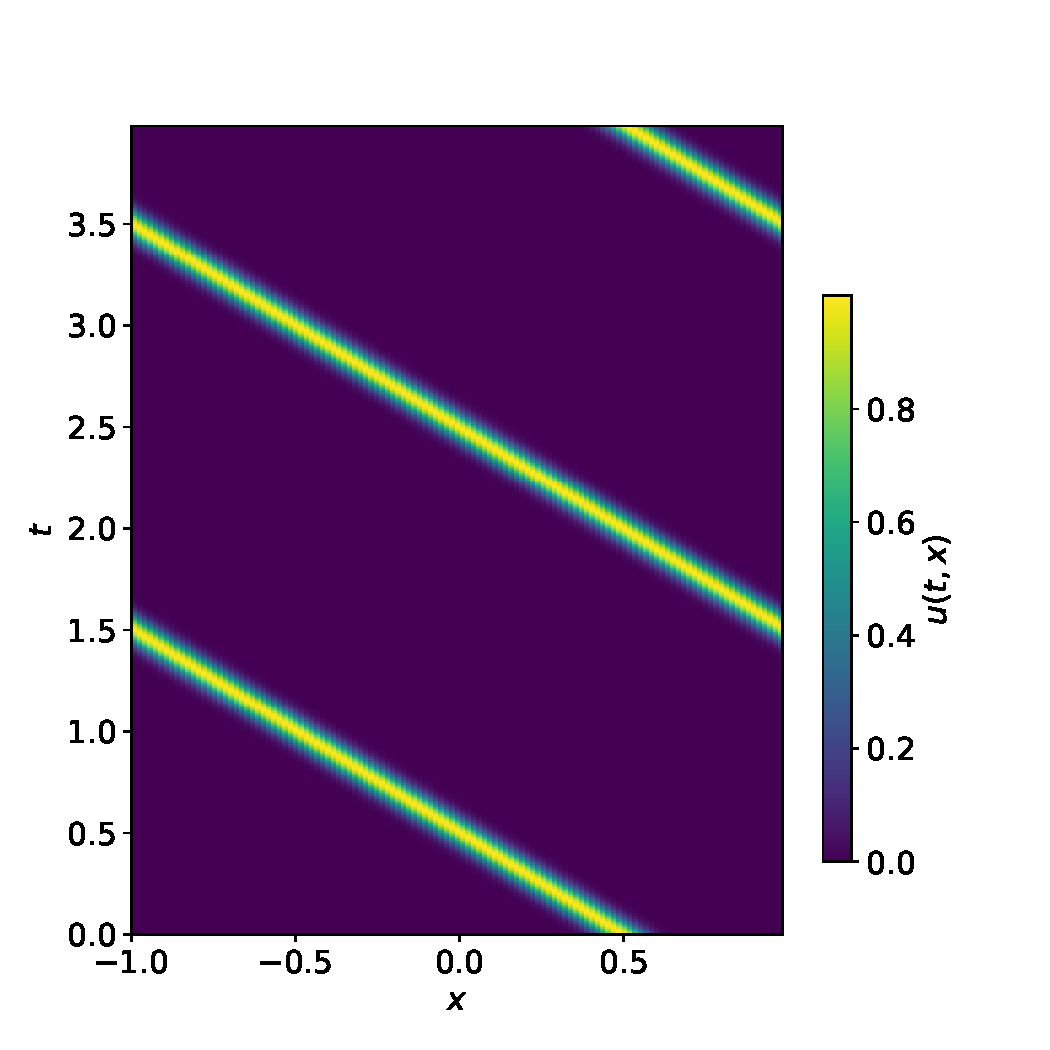
\includegraphics[width=0.8\textwidth]{1d_Wave_Solution2_u2.pdf}
  \caption{initial 2 Gaussian Pulse $u_2$}
\end{figure}
\pagebreak

그리고 두 pulse들을 합치는 코드를 작성하면 다음과 같다.
\begin{lstlisting}[language=Python]

fig, ax = plt.subplots(figsize=(7, 7), ncols=1)

combined= [i+j for i,j in zip(u_data_u1,u_data_u2)]
# plot the second solution on top of the first
pos1 = ax.imshow(combined, interpolation='none', origin='lower', cmap='viridis',
           extent=np.hstack(([xj[0], xj[-1]], [t_data_u1[0], t_data_u1[-1]])),
           aspect='auto')

fig.colorbar(pos1, ax=ax, location='right', anchor=(0, 0.3), shrink=0.7,
             label="$u(t, x)$")
ax.set_xlabel("$x$")
ax.set_ylabel("$t$")

plt.savefig("1D_Wave_Solution2_combined.pdf")

\end{lstlisting}
\begin{figure}[!ht]
  \centering
  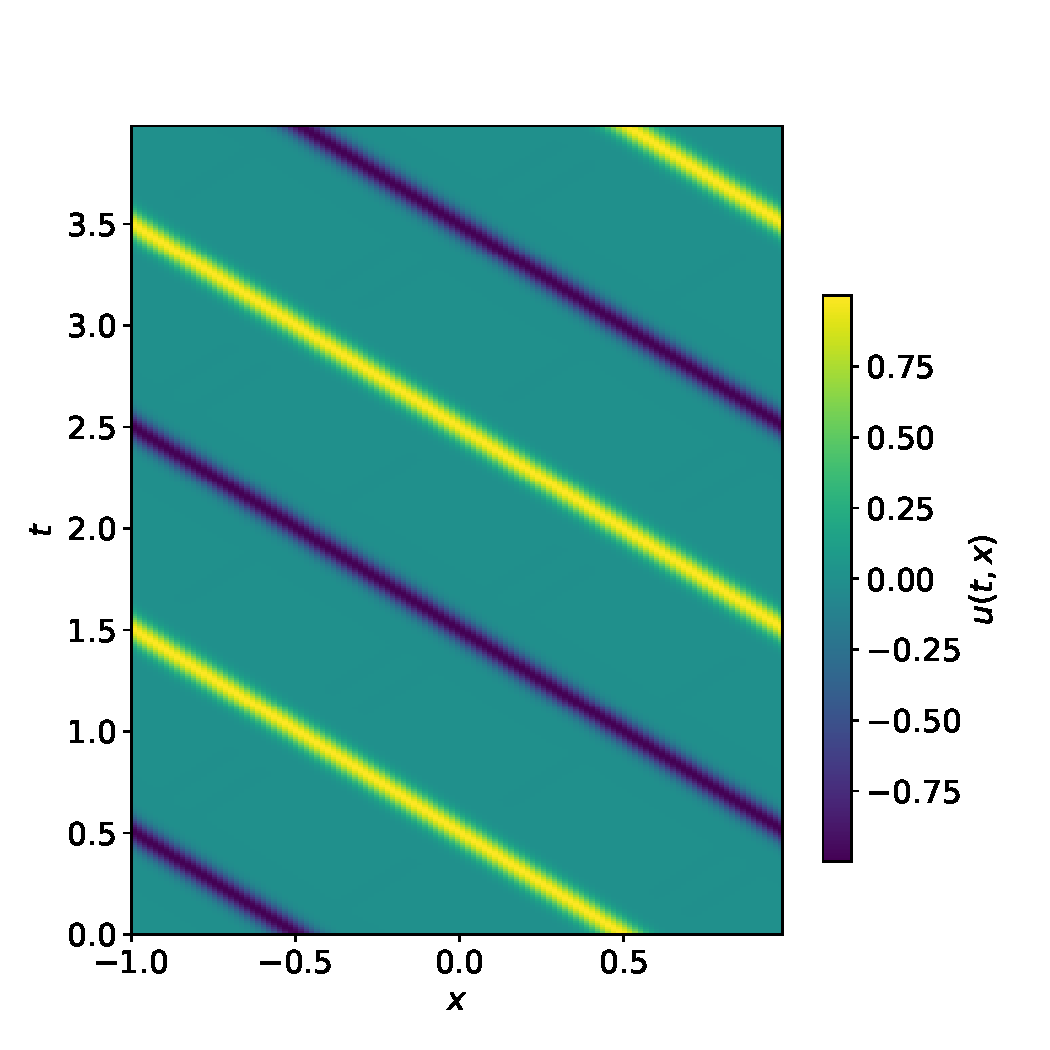
\includegraphics[width=0.8\textwidth]{1d_Wave_Solution2_combined.pdf}
  \caption{initial 2 Gaussian Pulse combined.pdf}
\end{figure}
\pagebreak

\subsection{Execution and Assessment}
두 pulse를 합치면, 새로운 pulse가 생성된다. 즉 이는 두 파동이 만나 진폭이 커진 경우로, 보강 간섭이 일어난 것이다. 만약 $u_1$ pulse가 왼쪽으로 $0.5$만큼 움직였을 경우에는 공명 현상이 일어나 파동이 상쇄되는 모습을 볼 수 있다. 예를 들어 $u_1$이 아래와 같이 되고, $u_2$ 데이터는 그대로 유지한채 두 그래프를 합치게 되면,
\begin{lstlisting}[language=Python]
uj = -1 * np.exp(-200 * (xj - 0.5)**2)            # - u(  0, x)
uj_old = -1 * np.exp(-200 * ((xj - 0.5) - dt)**2) # - u(-Dt, x)
\end{lstlisting}

\begin{figure}[!ht]
  \centering
  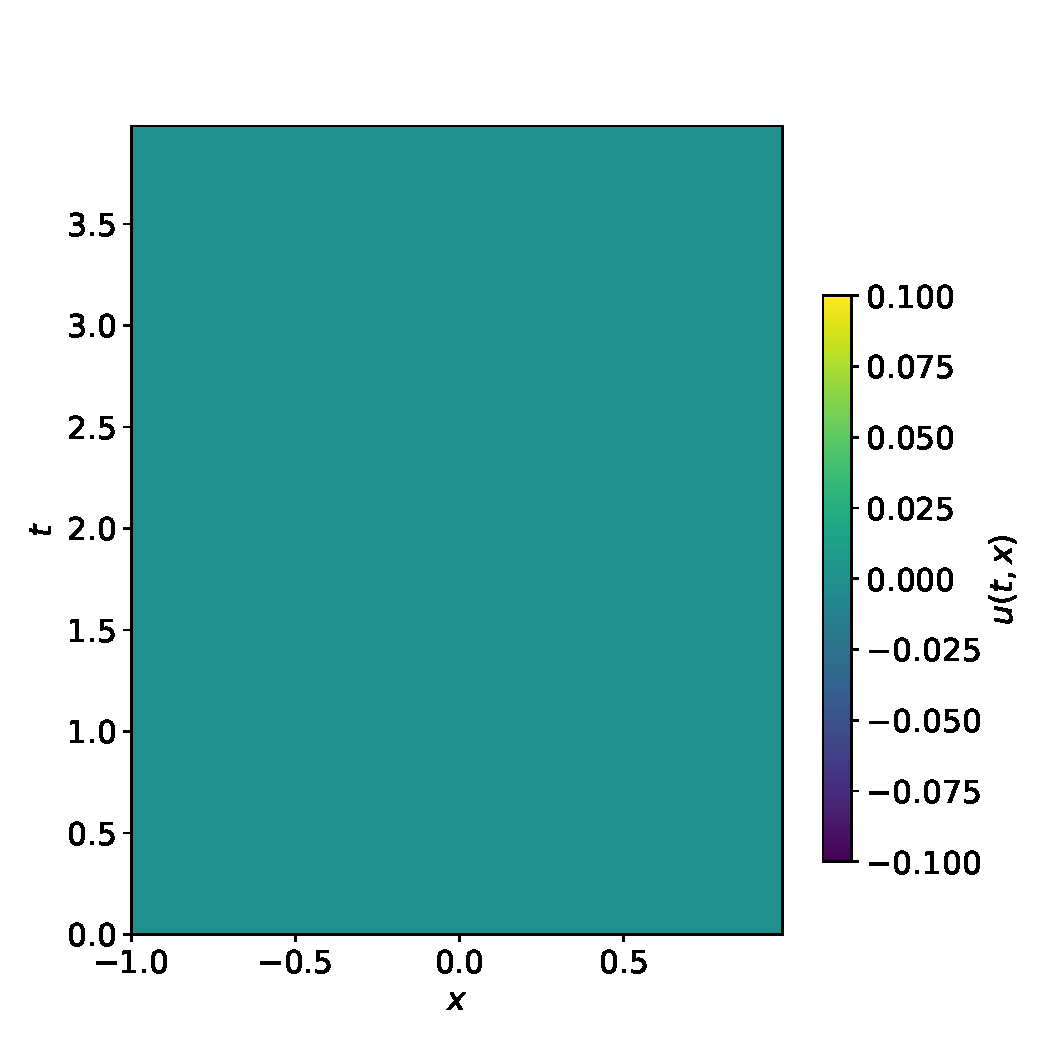
\includegraphics[width=0.8\textwidth]{1d_Wave_Solution2_combined2.pdf}
  \caption{initial 2 Gaussian Pulse combined resonance.pdf}
\end{figure}
이렇게 파동이 서로 영향을 끼치게 되면서 상쇄되는 모습을 볼 수 있다. 이는 곧, 진폭이 작아지거나 없어지는 경우이므로 상쇄 간섭이 일어난 것을 볼 수 있다.
\pagebreak









\section{1D Advection Solution}
\subsection{Problem Recognition} 
선행해서 배운 1D advection program에서 아래의 문제를 풀게끔 변경한다. 이때 다른 조건들은 선행해서 배운 조건과 동일하다.
\begin{equation}
\frac{\partial u}{\partial t} + c(x) \frac{\partial u}{\partial x} = -\frac{u}{5}
\end{equation}
그리고, 각 시간에서 $u$의 최대 진폭을 $t$의 함수로 표시한다. 최대 진폭이 $e^{-t/5}$처럼 감소하는 것을 알 수 있다. 이를 설명한다.
\subsection{Development of a solution} 
앞에서 배운 대류 방정식은 $x \in [0, 2\pi]$에서 주기적인 경계 조건을 가진다.
\begin{equation}
\frac{\partial u}{\partial t} + c(x) \frac{\partial u}{\partial x} = 0
,\qquad
c(x) = \frac{1}{5} + \sin^2(x - 1)
\end{equation}
이다. 그리고 초기 조건으로,
\begin{equation}
u(0, x) = \exp(-100 (x - 1)^2)
\end{equation}
을 가진다. 이때 우리는 DFT를 이용하여 공간을 미분할 것이고, 시간 미분은 leapfrog 공식을 따라 아래를 이용할 것이다.
\begin{equation}
u_t \approx \frac{u(t + \Delta t, x) - u(t - \Delta t, x)}{2\Delta t} = w(t, x)
\end{equation}
여기서 $w(t, x)$는 $-c(x)u_x$에 대한 추정값이다. 시작값 $u(-\Delta t, x)$을 얻기 위해서, 우리는 $x=1$일때의 파동 속도가 $v = c(1) = 1/5$라고 가정하여 $u(0,x)$에서 거꾸로 추정한다. 아래의 기존의 코드에서,

\begin{lstlisting}[language=Python]
N = 257 # number of grid points in x
xlim = [0, 2*np.pi] # bound of x
L  = xlim[1] - xlim[0]
xj = np.linspace(*xlim, N + 1)[:-1]
Dx = xj[1] - xj[0]
kj = np.hstack([
    np.arange(0,   N/2),     # k > 0 domain
    np.arange(-int(N/2), 0), # k < 0 domain
]) * 2*np.pi/L

dt = Dx / 8   # stability criterion is a whole different subject...
tmax = 8      # the maximum time to integrate
datadump_freq = int(0.05 / dt) # intermediate data dump frequency
outer_loop_count = int(tmax/dt / datadump_freq)

cj = .2 + np.sin(xj - 1)**2
uj = np.exp(-100 * (xj - 1)**2)             # u(  0, x)
uj_old = np.exp(-100 * (xj - 1 + .2*dt)**2) # u(-Dt, x)

# time and u data containers
t_data = [dt] * (1 + outer_loop_count)
u_data = [uj] * (1 + outer_loop_count)

for i in range(outer_loop_count):
    t_data[i] *= i * datadump_freq
    u_data[i]  = uj

    for _ in range(datadump_freq):
        Uj = fft.fft(uj)
        Wj = 1j*kj * Uj
        wj = fft.ifft(Wj).real
        uj_old, uj = uj, uj_old - 2*dt*cj*wj

t_data[-1] *= i * datadump_freq
u_data[-1]  = uj
\end{lstlisting}
이 코드의 18번째 줄 바로 아래의 식을 수정해야한다. 
\begin{equation}
u(-\Delta t, x) = \exp(-100 (x -1 + \frac{1}{5}dt)^2)
\end{equation}
이는, 우리가 선행해서 다룬 함수의 경우, $\frac{\partial u}{\partial t} + c(x) \frac{\partial u}{\partial x} = 0$ 이기 때문에, 위의 5번식
\begin{equation}
\frac{\partial u}{\partial t} + c(x) \frac{\partial u}{\partial x} = 0
\end{equation}
에서  $\frac{\partial u}{\partial t}$를 $u_t = dt$, $ \frac{\partial u}{\partial x}$를 $du$라고 두고, $dt$에 대하여 풀어주게 되면, 

\begin{equation}
dt + c(1)du  = 0
,\qquad
-dt = \frac{1}{5}du
\end{equation}
이기 때문에, t가 0일때,  $u(0,x)$에서 거꾸로 $u(-Dt, x)$를 유도해야 한다. 여기서 파동 방정식은 어떤 방정식도 $f(x \pm t)$로 쓰여진 방정식의 해로 쓰일 수 있기 때문에,  왼쪽 방향의 Pulse를 가지는 $u(-Dt, x)$에 대한 식을 적게 되면, 
\begin{equation}
u(-\Delta t, x) = \exp(-100 (x -1 + \frac{1}{5}dt)^2)
\end{equation}
을 구하게 되는 것이다. 하지만 이 문제의 경우, 10번의 식에서 우변이 0이 아닌 $-\frac{u}{5}$ 이기 때문에, 다시 위와 같이 dt에 대하여 풀어주게 되면
\begin{equation}
dt + \frac{1}{5}du  = -\frac{u}{5}
,\qquad
-dt = \frac{1}{5}du  + \frac{u}{5}
\end{equation}
그리고 이것을 대입시킨다.
\begin{equation}
u(-\Delta t, x) = \exp(-100 (x -1 + \frac{1}{5}dt + \frac{1}{5}u)^2)
\end{equation}
따라서, 코드를 수정하게 되면

\begin{lstlisting}[language=Python]
cj = .2 + np.sin(xj - 1)**2
uj = np.exp(-100 * (xj - 1)**2)              # u(  0, x)
uj_old = np.exp(-100 * (xj - 1 + .2*dt + .2 * uj)**2) # u(-Dt, x)
\end{lstlisting}

우리는 이제 각 시간에 따른 $u$의 최대 진폭을 구해야 한다. 이는 함수가 두개의 이중 for 문을 이용하여 각 시간에 따라 구해진 $u$의 리스트에서만 진폭의 최대값을 구하면 되므로, 이를 구현한 코드는 다음과 같다.

\begin{lstlisting}[language=Python]
N = 257 # number of grid points in x
xlim = [0, 2*np.pi] # bound of x
L  = xlim[1] - xlim[0]
xj = np.linspace(*xlim, N + 1)[:-1]
Dx = xj[1] - xj[0]
kj = np.hstack([
    np.arange(0,   N/2),     # k > 0 domain
    np.arange(-int(N/2), 0), # k < 0 domain
]) * 2*np.pi/L

dt = Dx / 8   # stability criterion is a whole different subject...
tmax = 8      # the maximum time to integrate
datadump_freq = int(0.05 / dt) # intermediate data dump frequency
outer_loop_count = int(tmax/dt / datadump_freq)



cj = .2 + np.sin(xj - 1)**2
uj = np.exp(-100 * (xj - 1)**2)              # u(  0, x)
uj_old = np.exp(-100 * (xj - 1 + .2*dt + .2 * uj)**2) # u(-Dt, x)

# time and u data containers
t_data = [dt] * (1 + outer_loop_count)
u_data = [uj] * (1 + outer_loop_count)

max_u = []
max_t = []
for i, index in enumerate(range(outer_loop_count)):
    t_data[i] *= i * datadump_freq
    u_data[i]  = uj
    

    max_t.append(t_data[i])
    max_u.append((abs(max(u_data[i]))- abs(min(u_data[i]))) / 2)
    
    for _ in range(datadump_freq):
        Uj = fft.fft(uj)
        Wj = 1j*kj * Uj
        wj = fft.ifft(Wj).real
        uj_old, uj = uj, uj_old - 2*dt*cj*wj

t_data[-1] *= i * datadump_freq
u_data[-1]  = uj

fig, ax = plt.subplots(figsize=(7, 7), ncols=1)


pos = ax.imshow(u_data, interpolation='none', origin='lower', cmap='viridis',
           extent=np.hstack(([xj[0], xj[-1]], [t_data[0], t_data[-1]])),
           aspect='auto')
fig.colorbar(pos, ax=ax, location='right', anchor=(0, 0.3), shrink=0.7,
             label="$u(t, x)$")
ax.set_xlabel("$x$")
ax.set_ylabel("$t$")


plt.savefig("Advection_solution.pdf")
\end{lstlisting}

\begin{figure}[!ht]
  \centering
  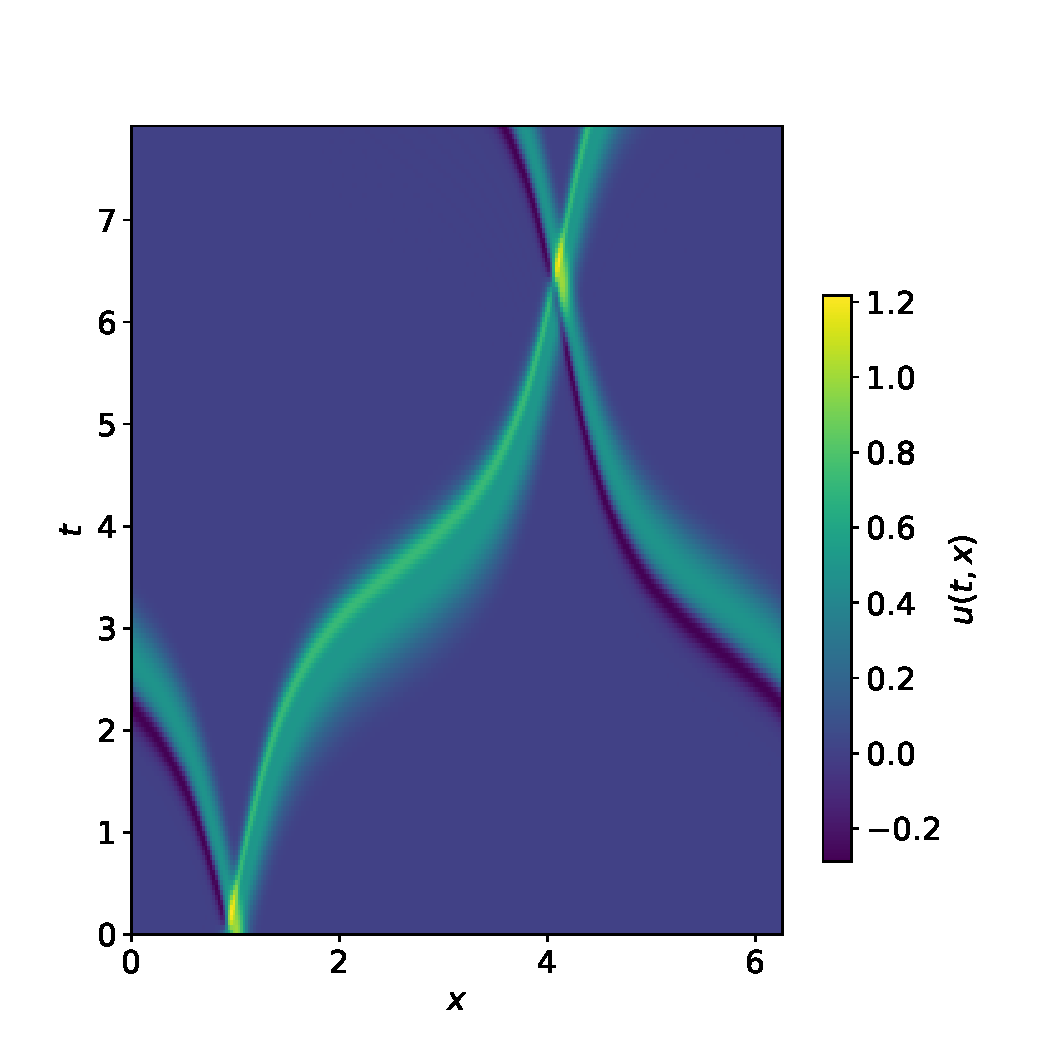
\includegraphics[width=0.8\textwidth]{Advection_solution.pdf}
  \caption{Advection Solution}
\end{figure}


그리고 최대 진폭을 나타낸 그림을 그리면
\begin{lstlisting}[language=Python]
plt.plot(max_t, max_u, '-r')
plt.savefig("maximum_amplitude.pdf")
\end{lstlisting}
\pagebreak
\begin{figure}[!ht]
  \centering
  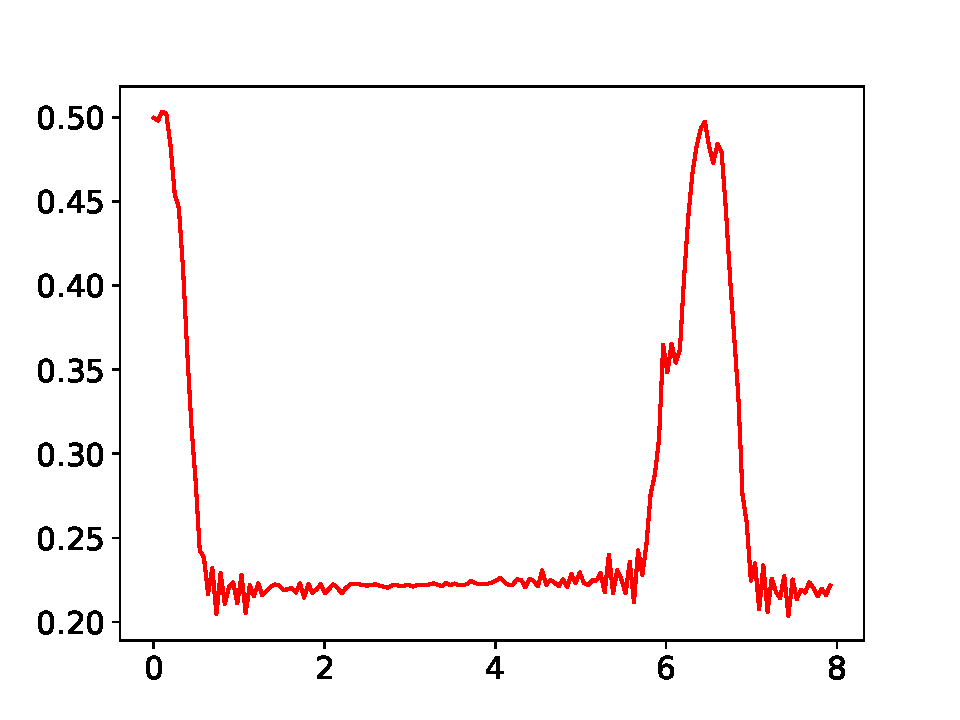
\includegraphics[width=0.8\textwidth]{maximum_amplitude.pdf}
  \caption{Maximum Amplitude}
\end{figure}



\pagebreak








\section{Do-Re-Mi-Fa-So-La-Ti-Do by FFT Module}
\subsection{Problem Recognition} 
note와 frequency, amplitude 가 주어졌을때, 첫음을 $C_4$를 기준으로 $Do-Re-Mi-Fa-So-La-Ti-Do$를 연주해야 한다. 앞서 배운 코드를 잠시 확인하면, 먼저 note와 frequency 그리고 amplitude 리스트를 정의한 후,  주파수와 진폭에 대한 그래프를 확인하면 다음과 같다.
\begin{figure}[!ht]
  \centering
  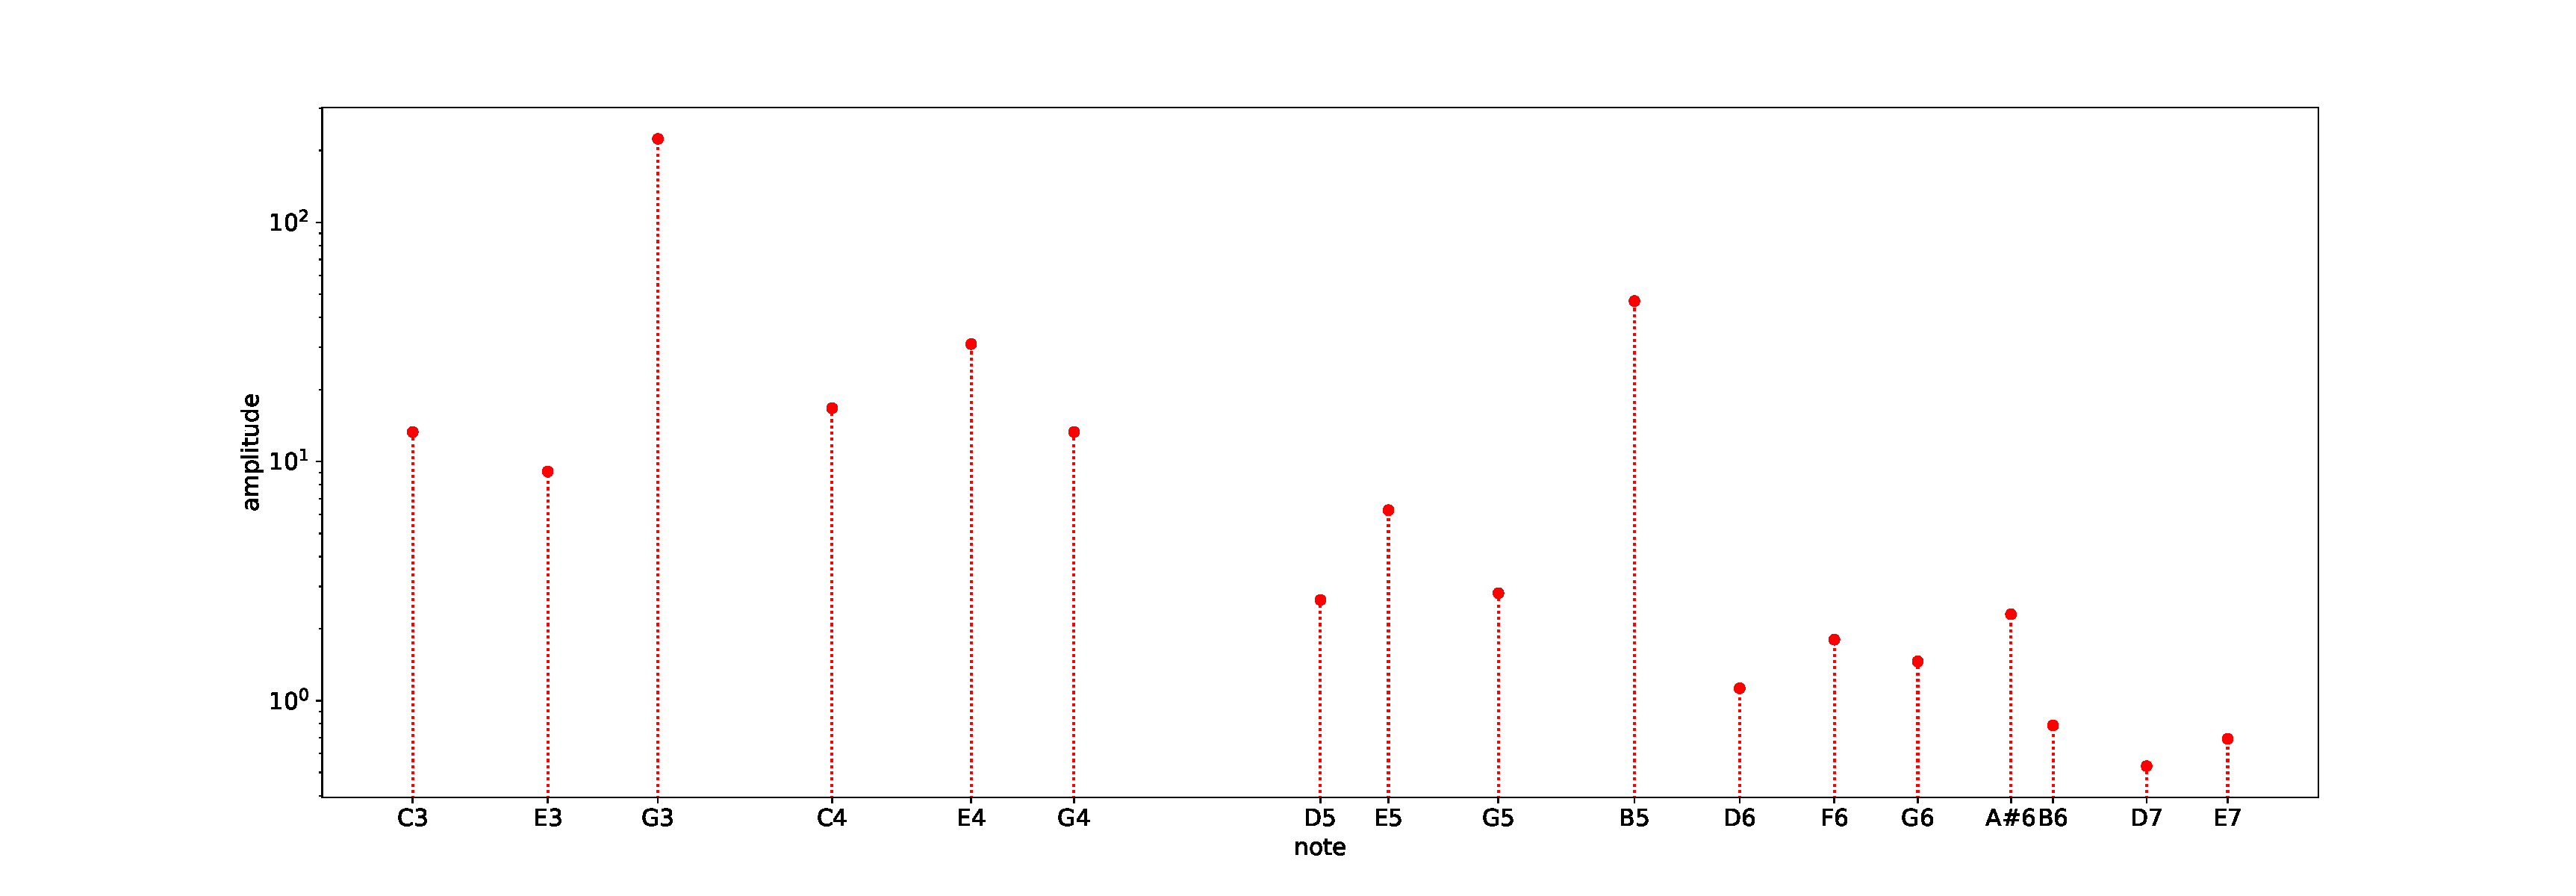
\includegraphics[width=1\textwidth]{example_DO.pdf}
  \caption{Example Amplitude - C Major}
\end{figure}
그리고 우리는,  아래의 식을 통하여, 코드의 2초 길이의 모노 오디오 샘플을 생성할 수 있다.
\begin{equation}
u(x) = \sum_{i = 1}^{N\ \text{notes}} A_i \cos(2\pi f_i t + \phi_i)
\end{equation}
이때, $A_i$ 그리고 $f_i$는 $i$번째 노트의 진폭과 주파수를 나타낸다. 또한 Phase Factor을 무작위의 $0 \le \phi_i < 2\pi$로 둠으로써, 코드를 연주할 수 있게 된다. 이를 이용하여, 우리가 원하는 음역대인 $C_4$에서 시작해 각각의 음에 따라 연속적이게 들리게 해야 한다. 
\subsection{Development of a solution} 
문제를 풀기 위해서, 우선 고려해야 할 것은 다음과 같다.
\begin{itemize}
    \item 오디오 샘플에서 원하는 도, 레 와 같은 각각의 사운드를 나타내야 한다.
    	\item 각각의 사운드를 만들 때에는, Filter을 이용하여 amplitude를 지우고, 그것을 위해서는 FFT를 이용하여야 한다.
    \item 나타낸 각각의 사운드를 합쳐 연속적인 사운드를 만들어야 한다.
    
\end{itemize}




선행된 예제에서는 Audio 함수를 사용했기 때문에, 마찬가지로 Audio 함수를 사용하여 오디오 샘플을 만들어 줄 것이다.  주어진 note에 따른 frequency와 amplitude에 대해, $B_3$부터 $C_{\sharp5}$까지의 음역대를 골랐다. 이를 각각의 리스트에 대해서 note, frequency 그리고 amplitude에 각각 넣어준뒤, note에 대한 amplitude의 그래프는 다음과 같다.

\begin{lstlisting}[language=Python]
note = ["B3", "C4", "C_shop4", "D4", "D_shop4", "E4", "F4", "F_shop4", "G4", 
        "G_shop4", "A4", "A_shop4", "B4", "C5", "C_shop5",
        
]
frequency = [ # in Hz
    246.94, 261.63, 277.18, 293.66, 311.13, 329.63, 349.23, 369.99, 392.00, 
    415.30, 440.00, 466.16, 493.88, 523.25, 554.37
]
amplitude = [
    139.71, 131.87, 124.47, 117.48, 110.89, 104.66, 98.79, 93.24, 88.01, 
    83.07, 78.41, 74.01, 69.85, 65.93,62.23
    
]

plt.figure(figsize=[30, 10])
ax = plt.subplot()
plt.loglog(frequency, amplitude, "or")
for x, y in zip(frequency, amplitude):
    plt.loglog([x, x], [0, y], ":r")
plt.xlabel("note")
plt.ylabel("amplitude")
plt.xticks(frequency, note)
ax.tick_params(axis='x', which='minor', bottom=False)
plt.savefig("B3_to_Cshop5_Figure1")
\end{lstlisting}

\begin{figure}[!ht]
  \centering
  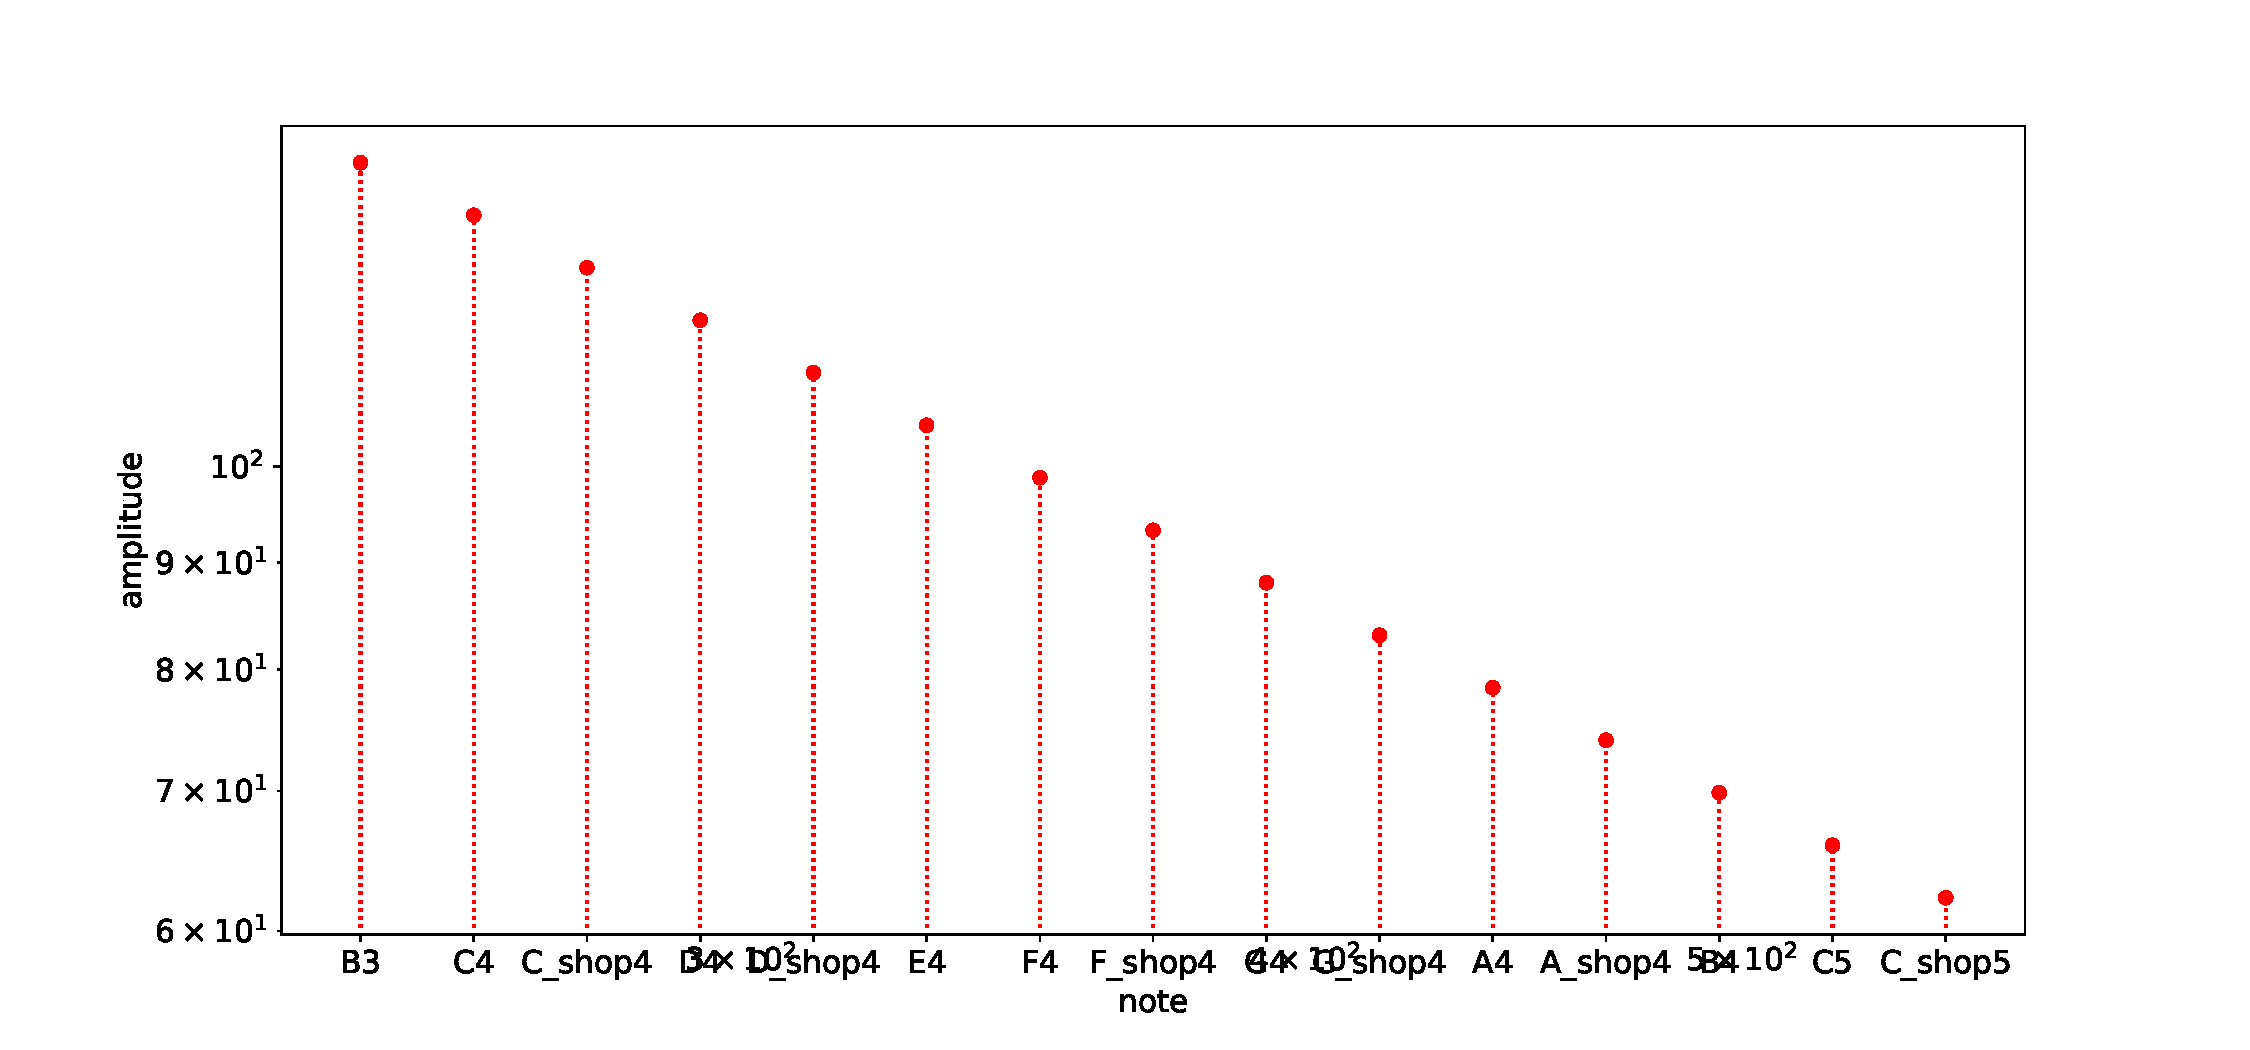
\includegraphics[width=1\textwidth]{B3_to_Cshop5_Figure1.pdf}
  \caption{$B_{3}$ to $C_{\sharp5}$  note and amplitude}
\end{figure}
\pagebreak
그리고 이 파형을 소리를 내려면, 우선 위 공식에 맞게 식을 세워주고, 무작위 위상에 대한 샘플을 만들 것이므로, random 함수를 사용하여 표현한다.

\begin{lstlisting}[language=Python]
# number of samples per second,
sampling_frequency = 48000 // 8

# then, maximum frequency that can be resolved
max_freq = 0.5 * sampling_frequency

# discrete time domain
max_time = 1 # in seconds
time = np.linspace(0, max_time, sampling_frequency * max_time + 1)[:-1]

# random phases for different notes
phase = np.random.rand(len(time)) * 2*np.pi

# wave samples
wave  = sum(A * np.cos(2*np.pi*f*time + ph) 
            for A, f, ph in zip(amplitude, frequency, phase))
\end{lstlisting}
이렇게까지 하면 우리는 위에서 정한,  $B_3$부터 $C_{\sharp5}$까지의 음역대의 모든 wave가 재생이 될 것이다. 하지만 우리는 순차적으로 연속적인 도레미파 솔라시도의 소리를 원하기 때문에, 나머지 파장대의 소리를 제거할 필요가 있다.

우선, 도 라는 소리를 내기 위해서는 도 이외에 모든 파장대의 소리를 제거해야 한다. 그러기 위해선, 먼저 FFT를 통해 푸리에 함수로 만들어 준다.

\begin{lstlisting}[language=Python]
Wj = fft.fft(wave)
N  = len(Wj)

Dk = 2*np.pi / (max(time) - min(time))
kj = np.hstack([
    np.arange(0,   N/2),     # k > 0 domain
    np.arange(-int(N/2), 0), # k < 0 domain
]) * Dk

# kj is 'angular' frequency.
# divide it by 2pi to convert to frequency in Hz
fj = kj / (2*np.pi)

# power spectral density
Pj = np.abs(Wj/N)**2 / Dk

plt.figure(figsize=[30, 10])
ax = plt.subplot()
plt.loglog(fj[:int(N/2)], Pj[:int(N/2)], "-r", lw=1)
plt.xlim([frequency[0]*0.8, frequency[-1]*1.2])
plt.xlabel("note")
plt.ylabel("$P(k)$")
plt.xticks(frequency, note)
ax.tick_params(axis='x', which='minor', bottom=False)
plt.grid(axis="x")
plt.savefig("FFT_figure.pdf")
\end{lstlisting}

\begin{figure}[!ht]
  \centering
  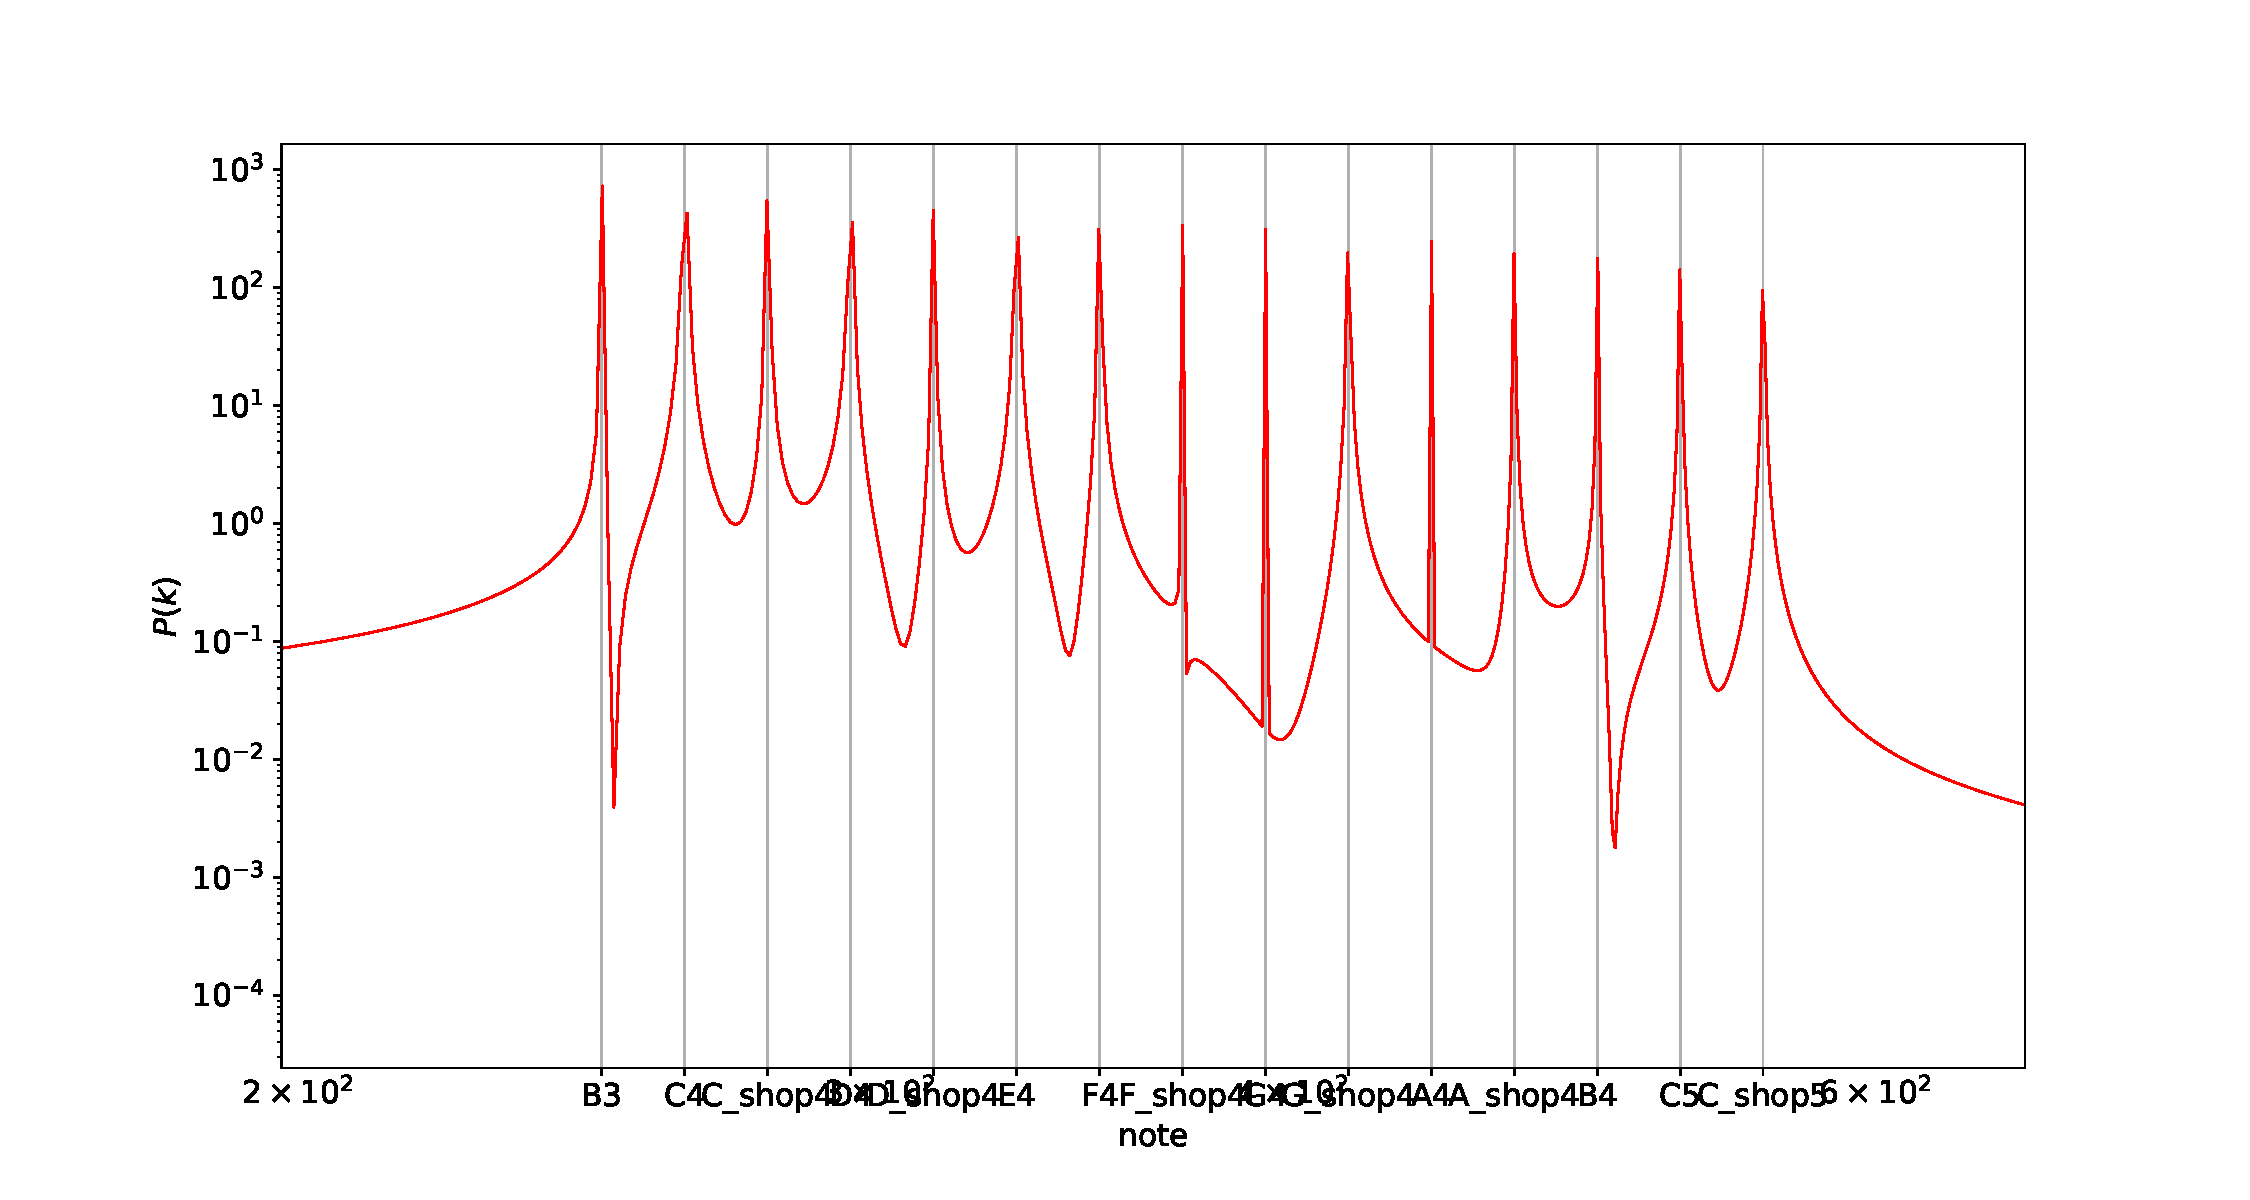
\includegraphics[width=1\textwidth]{FFT_figure.pdf}
  \caption{$B_{3}$ to $C_{\sharp5}$  note and amplitude}
\end{figure}

\pagebreak
우리는 "도"의 음역대를 원하기 때문에,  Filter을 이용하여 도를 제외한 wave amplitude는 제거하고, 역변환 시켜야 한다. 여기까지 코드를 작성하면 다음과 같다.
\begin{lstlisting}[language=Python]
Major = ["C4", "D4", "E4","F4", "G4", "A4", "B4", "C5",]

def Filter(index):
        freq_cut1 = 0.5 * (frequency[index] + frequency[index + 1])
        freq_cut2 = 0.5 * (frequency[index - 1] + frequency[index])
        indices1 = np.abs(fj) > freq_cut1
        indices2 = np.abs(fj) < freq_cut2
        filtered_Wj = Wj.copy()
        filtered_Wj[indices1,] *= 0
        filtered_Wj[indices2,] *= 0   
        return fft.ifft(filtered_Wj).real        
\end{lstlisting}
위 Filter 함수는, 우리가 원하는 음에 해당하는 

\begin{lstlisting}[language=Python]
note = [
     "C3",  "E3",  "G3",  "C4",  "E4",   "G4",   "D5",   "E5",   "G5",
     "B5",  "D6",  "F6",  "G6", "A#6",   "B6",   "D7",   "E7",
]
\end{lstlisting}
note 리스트의 해당 index를 입력시키게 되면, 그 음을 제외한 모든 wave amplitude를 제거하는 함수이다. 이렇게 까지 하여, 도라는 음역대를 재생할 수 있게 되었다.

나머지 소리를 연속해서 내기 위해서는, 반드시 wave 하나에 우리가 담고자 하는 $Do-Re-Mi-Fa-So-La-Ti-Do$ wave 파형이 다 들어있어야 하는데, 따라서 이 함수를 각각의 레, 미, 파, ... , 도($C_5$)까지 반복시킬 필요가 있다. 하지만, 문제는 Audio 파일에는 하나의 wave만 담을 수 있기 때문에, 여러개의 소리를 덧붙일려면 일반적인 합의 방식을 사용하면 안된다. 우선 우리가 구한 이 wave 변수는 1차원 array로 이루어져 있는데 여기서 array를 그저 더하게 되면 wave amplitude는 모든 음역대의 소리가 합쳐지게 된다. 이를 좀더 구체화 시키면,

\begin{lstlisting}[language=Python]
filtered_wave1 = Filter(1)
#x = np.linspace(0, time, len(filtered_wave1))
plt.figure(figsize = (9, 9))
plt.plot(time, filtered_wave1, '.r', label = '$C_4$ wave')
plt.legend()
plt.grid()
plt.xlabel("time")
plt.ylabel("wave amplitude value")
plt.savefig("wave_amp_C4.pdf")
\end{lstlisting}

\begin{figure}[!ht]
  \centering
  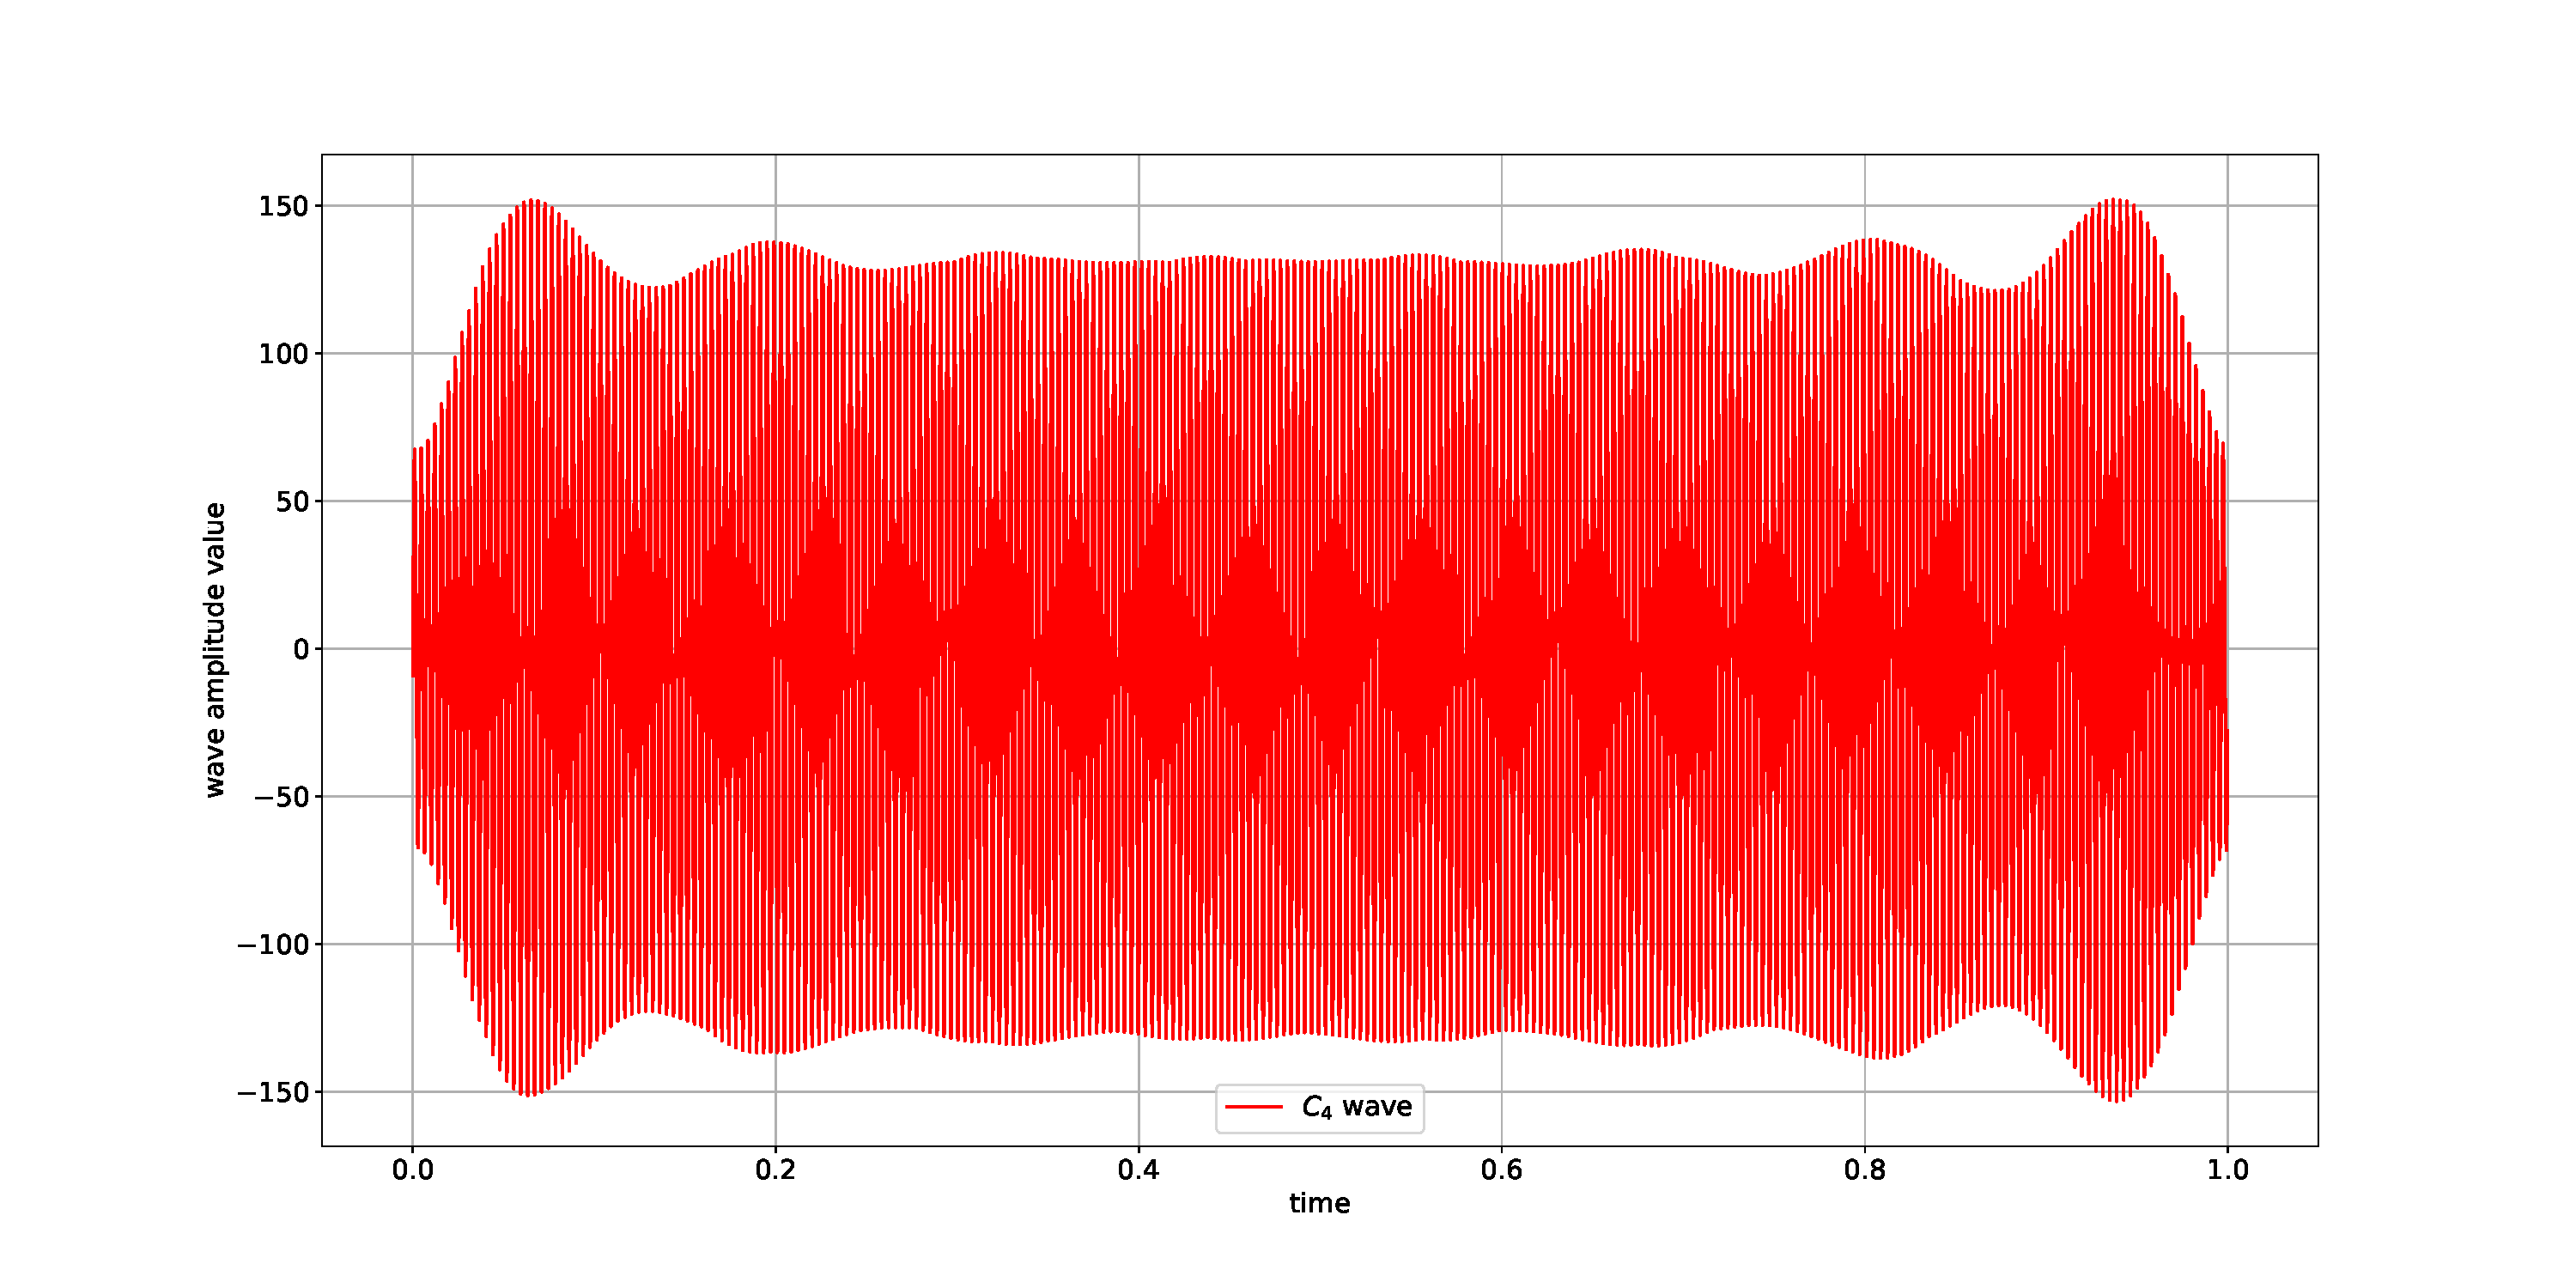
\includegraphics[width=1\textwidth]{wave_amp_C4.pdf}
  \caption{$C_{4}$ amplitude}
\end{figure}

\pagebreak

우리가 구한 도에 대한 wave amplitude를 $t=0$에서 1까지를 보여준 그래프이다. 이때, 위상이 여러개로 보이는 이유는 우리가 0 에서 $2\pi$까지 무작위로 만들어진 위상에 대한 그래프이기 때문에 여러개의 amplitude wave를 볼 수 있게 된다. 여기서 만약, 합의 방식으로 함수를 더하게 되버리면, 소리를 들어보면, 도와 레가 합쳐진 소리가 들리게 되는데, 실제로 그래프를 그려보면,

\begin{lstlisting}[language=Python]
filtered_wave1 = Filter(1)
filtered_wave3 = Filter(3)
#x = np.linspace(0, time, len(filtered_wave1))
plt.figure(figsize = (9, 9))
plt.plot(time, filtered_wave1, '.r', label = '$C_4$ wave')
plt.plot(time, filtered_wave3, '.b', label = '$D_4$ wave')
plt.legend()
plt.grid()
plt.xlabel("time")
plt.ylabel("wave amplitude value")
plt.savefig("wave_amp_C4+D4.pdf")
\end{lstlisting}

\begin{figure}[!ht]
  \centering
  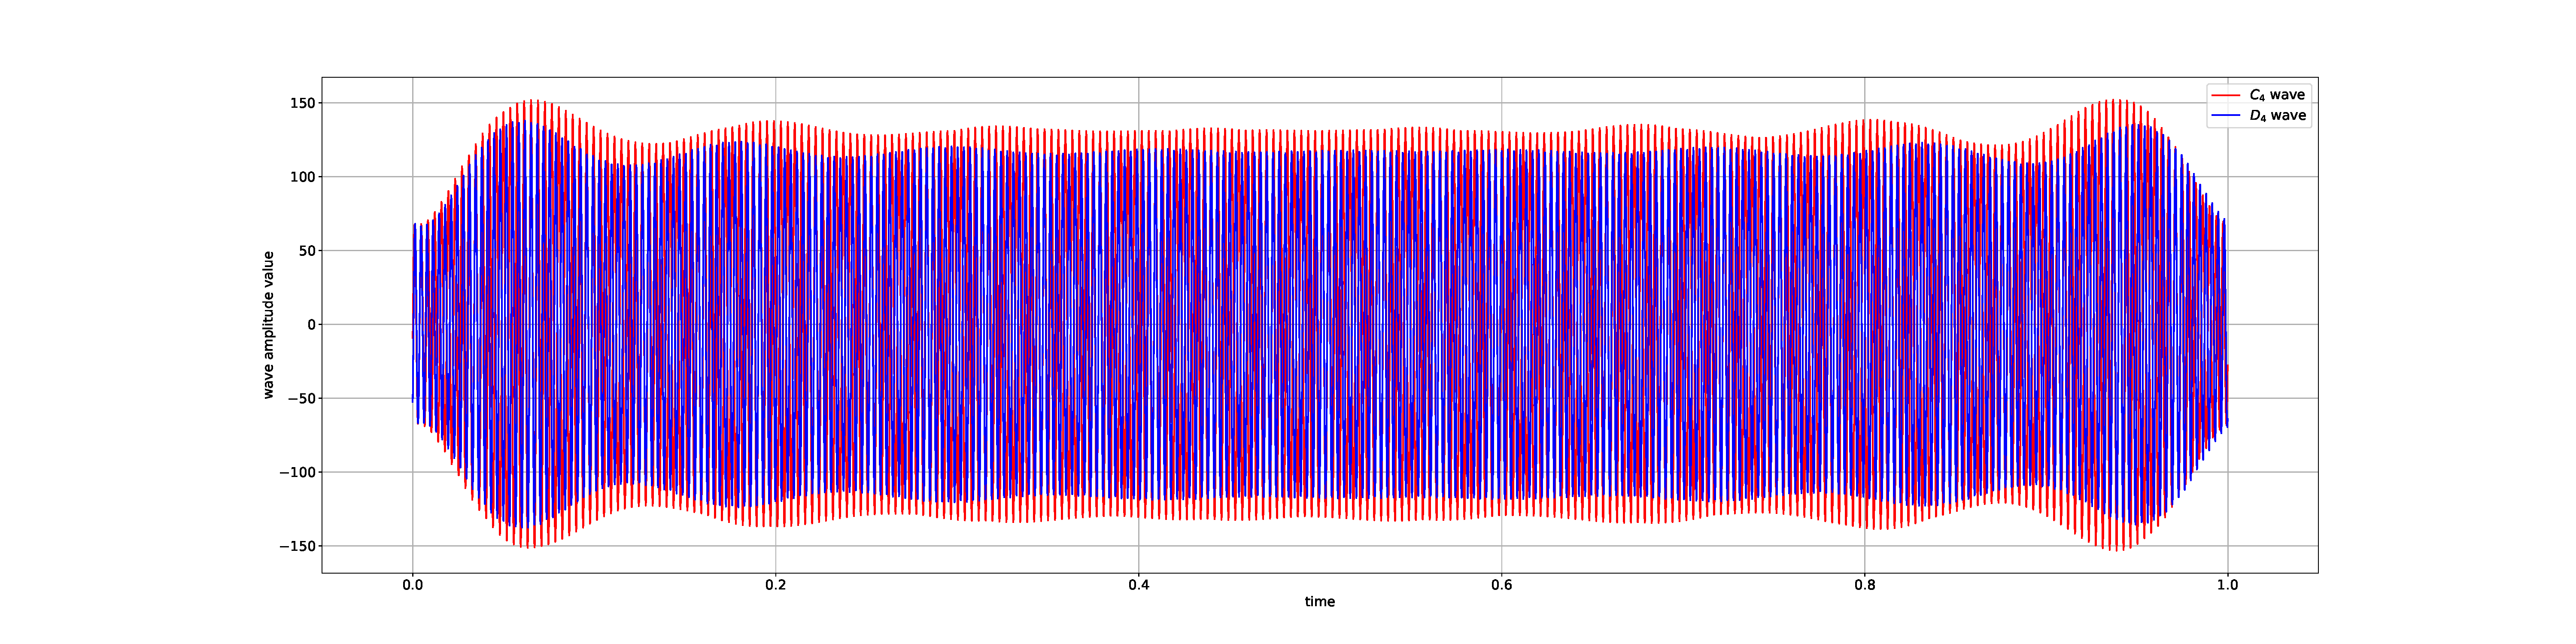
\includegraphics[width=1\textwidth]{wave_amp_C4+D4.pdf}
  \caption{$C_{4}$ + $D_{4}$ amplitude}
\end{figure}

두 파장대의 amplitude wave 가 합쳐져 각각의 소리를 연속적으로 내지 않고, 한번에 재생되게 되면서 새로운 wave가 형성되게 된다. 따라서 소리를 듣게 되면, 도와 레가 합쳐진 소리를 들을 수 있게 된다. 각각의 파장을 연속적으로 재생시키려면 겹치지 않게 wave를 각각 이어주어야 한다. 우리가 앞서 봤듯, wave는 1D array로 되어있기 때문에, 이를 이어주기 위해서는 np.concatenate를 이용하고, 이때 이어주는 방향은 axis = 0 으로 x축 방향으로 파장을 시간에 따라 붙여주면 된다. 따라서 우리는 도와 레의 amplitude wave를 붙여준 것을 그래프로 확인하게 되면,

\begin{lstlisting}[language=Python]
filtered_wave1 = Filter(1)
filtered_wave3 = Filter(3)

filtered_wave_sum = np.concatenate((filtered_wave1, filtered_wave3), axis = 0)

# time
x_sum = np.linspace(0, 2 * max_time, 2 * (sampling_frequency * max_time + 1) - 1)[:-1]
x_C4 = time
x_D4 = np.linspace(1, 2, (sampling_frequency * max_time))

# plot C4 + D4
plt.figure(figsize = (20, 10))
plt.plot(x_sum, filtered_wave_sum, ':k', label = '$C_4$ + $D_4$ wave', alpha = 0.5) 
plt.plot(x_C4, filtered_wave1, '.r', label = '$C_4$ wave', alpha = 0.25)
plt.plot(x_D4, filtered_wave3, '.b',  label = '$D_4$ wave',
         alpha = 0.25)
plt.legend()
plt.grid()
plt.xlabel("time")
plt.ylabel("wave amplitude value")
plt.savefig("wave_amp_independence.pdf")
Audio(filtered_wave_sum, rate=sampling_frequency)
\end{lstlisting}

\begin{figure}[!ht]
  \centering
  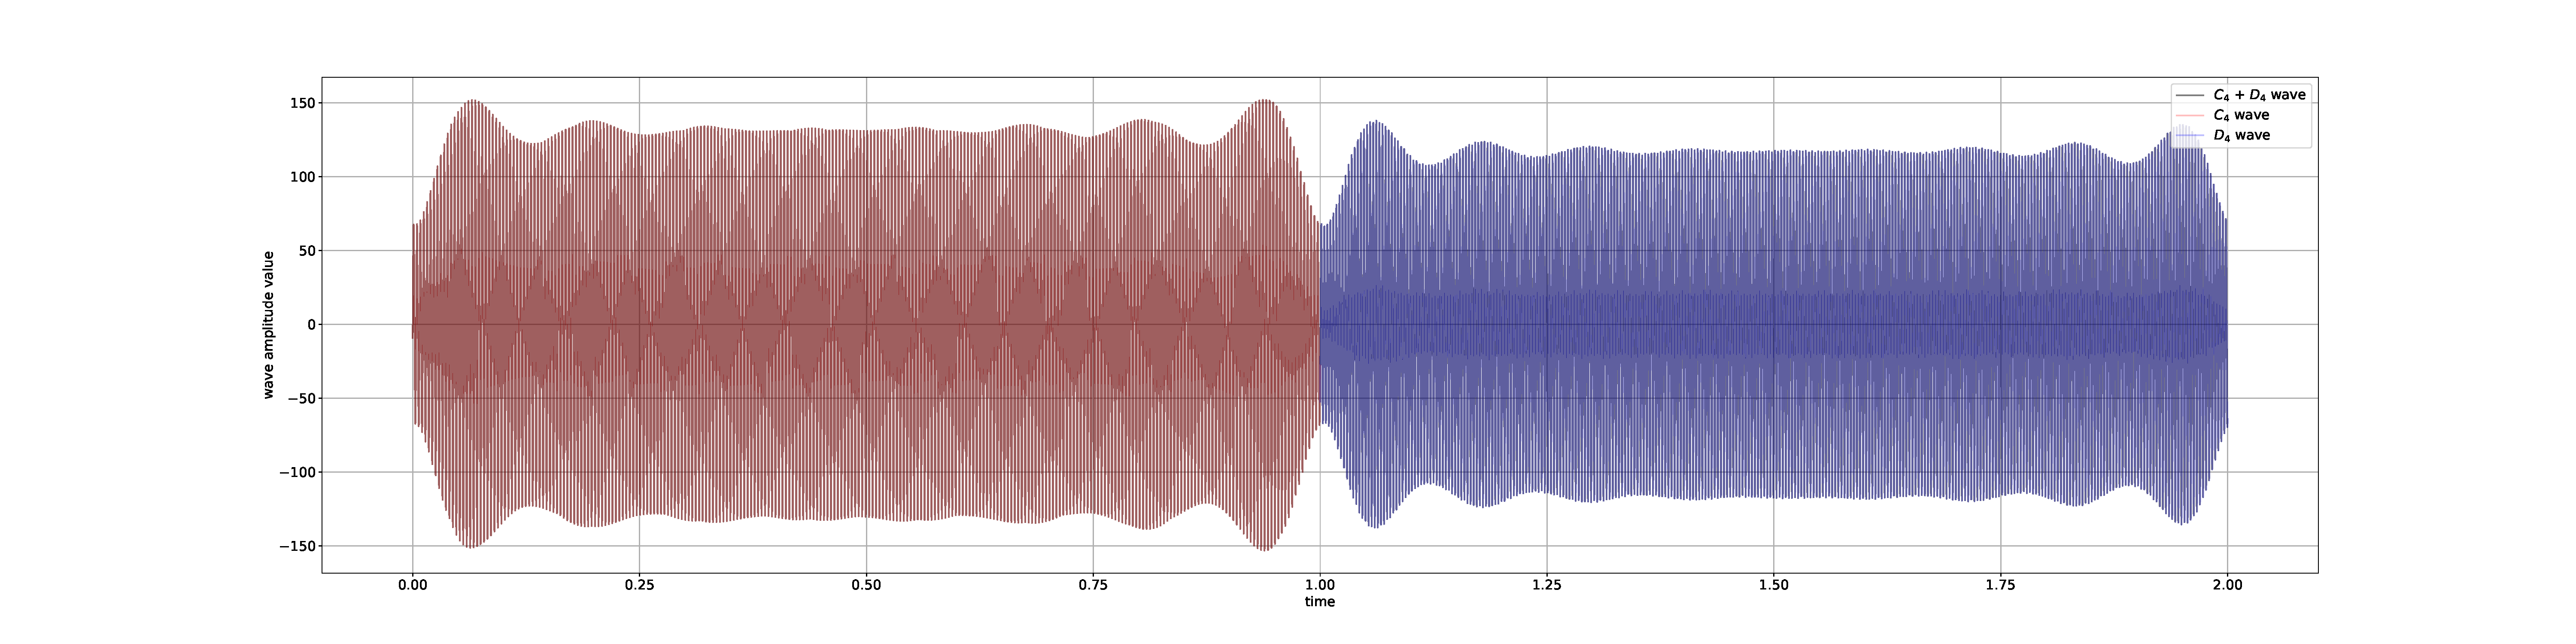
\includegraphics[width=1\textwidth]{wave_amp_independence.pdf}
  \caption{$C_{4}$ + $D_{4}$ independece amplitude}
\end{figure}


우리가 예상했던대로, np.concatenate를 이용하면 빨간색과 파란색 두 파장이 겹치지 않게 시간 $t = 1$일때, $D_4$에 해당하는 wave amplitude가 합쳐지면서, 하나의 검은 새로운 wave amplitude가 만들어 진 것을 볼 수 있으며, 시간에 대해 각각 독립적이게 연속적인 형상을 띄는 것을 볼 수 있다. 또한, Audio 함수를 통하여 직접 듣게 되면, 우리가 원하는 도, 레 의 독립적이고 연속적인 사운드를 들을 수 있다. 우리는 이것을 통하여 실제 Audio wave에도 적용한다.

\begin{lstlisting}[language=Python]
# array box
filtered_wave_sum = np.zeros(1)

# filtered code put in box
for code in Major:
    index = [i for i, n in enumerate(note) if n == code][0]

    # Filtering 
    filtered_wave = Filter(index)
    filtered_wave_sum = np.concatenate((filtered_wave_sum, filtered_wave), axis = 0)

Audio(filtered_wave_sum, rate=sampling_frequency)
\end{lstlisting}
fitered wave sum 변수를 먼저 빈 1차원의 array로 만들어 준 뒤, 우리가 Filter을 통해 만든 각각의 wave amplitude를 np.concatenate를 통하여 이어주고, 최종적으로 만들어진 fitered wave sum를 재생하면, 하나의 오디오에서 연속적인 음을 나타낼 수 있게 된다. 

\subsection{Execution and Assessment}
우리는 원하는 사운드를 얻기위해 FFT로 변환시켜 푸리에 함수로 구한 뒤, Filter을 적용함으로써 역변환 시켜 원하는 사운드를 얻는 문제를 풀어보았다. 또한 우리가 원하고자 하는 wave amplitude는 파형을 더하거나 독립적이게 array에서 합하게 해줌으로써, 만약 원한다면 화음이나, 독립적인 사운드를 내는 방식도 가능한 것을 확인하였다.































































































































































































































































































































































































































































































































































































\end{document}
